%Typeset using XeLaTeX

\documentclass[10pt,a4paper]{book}
%
%
\usepackage{amsmath,amssymb,amsthm}
\usepackage{phonetic}
\usepackage{fancyhdr}
\usepackage[pass]{geometry}
\usepackage{fontspec}
\usepackage{url}
\usepackage{booktabs}
\usepackage[table,xcdraw,dvipsnames]{xcolor}
\usepackage{algorithm}
\usepackage{algorithmicx}
\usepackage{algpseudocode}

\usepackage{wrapfig}  %% package needed for pictures to be wrapped up in text.
\usepackage{float} %% adds the [H] option in the figure environment.
\usepackage{tcolorbox}  %% frames.
\usepackage{moreenum} %% more enumeration options i guess.. i need it for /greek option.
\usepackage[toc,page]{appendix}
\usepackage[super]{nth}
\usepackage{epigraph} %% quotes in chapters
\usepackage{graphicx}
\usepackage[font=itshape]{quoting}
\usepackage{subfloat}

\usepackage[backend=bibtex,style=numeric,sorting=sortkey]{biblatex}
\addbibresource{myBibliography.bib}
\defbibfilter{papers}{
  type=article or
  type=inproceedings or
  type=book or
  type=unpublished
}

\usepackage{xunicode}
\usepackage{xltxtra}
%\usepackage{xgreek}
\setmainfont[Mapping=TeX-text]{Times New Roman}
%
\usepackage[Glenn]{fncychap}
\ChNameVar{\bfseries\Large}
\usepackage{tabularx}
\usepackage[normalem]{ulem}

%% myPackages (Extra)
\usepackage{enumitem}

\usepackage{bookmark}

\renewcommand{\maketitle}{
  \begin{titlepage}
    \newgeometry{left=4cm, top=2.3cm, bottom=2.3cm}

    \hbox{
      \mbox{ \hspace{-1.3cm} }
      \vrule depth 0.98 \textheight
      \mbox{ \hspace{1cm} }

        \vtop{
          \vspace{2cm}

          \begin{flushleft}
            \huge{\bf \TITLOS\\}
            \vskip3cm
            \Large  \ONOMA\\
            \REGNUM\\
            \vskip3cm

            \begin{minipage}{8.5cm}
              \begin{flushleft}
                \normalsize {\it {\bf Examination committee:}\\
                \PRONE\\
                \vskip0.2cm
                \PRTWO\\
                \vskip0.2cm
                \PRTHREE}
              \end{flushleft}
            \end{minipage}

            \vskip0.2cm
            \hskip0.5cm
            \begin{minipage}{6cm}
              \begin{flushleft}
                \normalsize {\it {\bf Supervisor:}\\
                \SPNAME, \SPRANK, \\ \SPDEPART,\\
                \SPINSTI.\\
                }
              \end{flushleft}
            \end{minipage}

          \end{flushleft}

          \vskip4cm
          \hskip4.5cm
          \begin{minipage}{5cm}
            \begin{center}
              \includegraphics[width=0.8\textwidth]{alma.png}
            \end{center}
          \end{minipage}
        }
    }

 \end{titlepage}
 }

 %%%%%%%%%%%%%%%%%%%%%%%%%%%%%%%%%%%%%%%%%%%%%%%%%%%%%%%%%%%%%%%%%%%%%%%%
 %%%%%%%%%%%%%%%%%%%%%%%%%%%%%%%%%%%%%%%%%%%%%%%%%%%%%%%%%%%%%%%%%%%%%%%%

\theoremstyle{definition}
\newtheorem{ex}{}[section]
\newtheorem{definition}{Definition}[chapter]
\newtheorem{theorem}[definition]{Theorem}
\newtheorem{lemma}[definition]{Lemma}
\newtheorem{corollary}[definition]{Corollary}
\theoremstyle{remark}
\newtheorem{example}[definition]{Example}
\newtheorem{claim}[definition]{Claim}

%%%%%%%%%%%%%%%%%%%%%%%%%%%%%%%%%%%%%%%%%%%%%%%%%%%%%%%%%%%%%%%%%%%%%%%%%
%%%%%%%%%%%%%%%%%%%%%%%%%%%%%%%%%%%%%%%%%%%%%%%%%%%%%%%%%%%%%%%%%%%%%%%%%

\fancyhead[LO]{\slshape \leftmark}
\fancyhead[RE]{\slshape \rightmark}
\fancyhead[LE]{}
\fancyhead[RO]{}
\fancyfoot[LO,RE]{
\tiny{\it}}

%%%%%%%%%%%%%%%%%%%%%%%%%%%%%%%%%%%%%%%%%%%%%%%%%%%%%%%%%%%%%%%%%%%%%%%%%
%% This is for code environment, helpful.
%% (not complete, I didn't need everything)
%%%%%%%%%%%%%%%%%%%%%%%%%%%%%%%%%%%%%%%%%%%%%%%%%%%%%%%%%%%%%%%%%%%%%%%%%
\def\code#1{\texttt{#1}}
\newcommand{\easyfigure}[3]{
  \begin{figure}
    \centering
    \includegraphics[width=0.9\columnwidth,keepaspectratio]{figures/#2.#1}
    \caption{#3}
    \label{fig:#2}
  \end{figure}
}
%%%%%%%%%%%%%%%%%%%%%%%%%%%%%%%%%%%%%%%%%%%%%%%%%%%%%%%%%%%%%%%%%%%%%%%%%
%% Bitcoin font!! haha..
%%%%%%%%%%%%%%%%%%%%%%%%%%%%%%%%%%%%%%%%%%%%%%%%%%%%%%%%%%%%%%%%%%%%%%%%%
\def\bitcoin{%
  \leavevmode
  \vtop{\offinterlineskip %\bfseries
    \setbox0=\hbox{B}%
    \setbox2=\hbox to\wd0{\hfil\hskip-.03em
    \vrule height .3ex width .15ex\hskip .08em
    \vrule height .3ex width .15ex\hfil}
    \vbox{\copy2\box0}\box2}}

%%%%%%%%%%%%%%%%%%%%%%%%%%%%%%%%%%%%%%%%%%%%%%%%%%%%%%%%%%%%%%%%%%%%%%%%%
%% Footnote in verbatim
%%%%%%%%%%%%%%%%%%%%%%%%%%%%%%%%%%%%%%%%%%%%%%%%%%%%%%%%%%%%%%%%%%%%%%%%%
  \newcommand{\vfchar}[1]{%
  % the usual trick for using a "variable" active character
  \begingroup\lccode`~=`#1 \lowercase{\endgroup\def~##1~}{%
  % separate the footnote mark from the footnote text
  % so the footnote mark will occupy the same space as
  % any other character
  \makebox[0.5em][l]{\footnotemark}%
  \footnotetext{##1}%
  }%
  \catcode`#1=\active
  }
  \newenvironment{fverbatim}[1]
  {\verbatim\vfchar{#1}}
  {\endverbatim}

%%%%%%%%%%%%%%%%%%%%%%%%%%%%%%%%%%%%%%%%%%%%%%%%%%%%%%%%%%%%%%%%%%%%%%%%%
%% Spliting bibliography
%%%%%%%%%%%%%%%%%%%%%%%%%%%%%%%%%%%%%%%%%%%%%%%%%%%%%%%%%%%%%%%%%%%%%%%%%
%\begin{category}[A]{First category}
%  \SBentries{signal,montgomery}
%\end{category}
%\begin{category}[B]{Second category}
%  \SBentries{edward,curve25519}
%\end{category}

\usepackage{hyperref}
\hypersetup{
    colorlinks=true,       % false: boxed links; true: colored links
    linkcolor=blue,          % color of internal links (change box color with linkbordercolor)
    citecolor=red,        % color of links to bibliography
    filecolor=magenta,      % color of file links
    urlcolor=cyan           % color of external links
}

%
%
\begin{document}
%
%
%% First page
%
\newcommand{\ONOMA}{Orestis Konstantinidis}
\newcommand{\TITLOS}{Monero mining: CryptoNight Analysis}
\newcommand{\REGNUM}{AL1180006}
%%
\newcommand{\PRONE}{Prof. Dr. Aggelos Kiayias, Department of Informatics and Telecommunications, NKUA.}
\newcommand{\PRTWO}{Professor's name, Department or School, Institution.}
\newcommand{\PRTHREE}{Professor's name, Department or School, Institution.}

\newcommand{\SPNAME}{Dr. Aggelos Kiayias}
\newcommand{\SPRANK}{Associate Professor}
\newcommand{\SPDEPART}{Department of Informatics and Telecommunications}
\newcommand{\SPINSTI}{National and Kapodistrian University of Athens}
%%%
\maketitle
\clearpage
%
%% Empty page
%
\thispagestyle{empty}
\null
\clearpage

\input{secondPage.tex}
%
%%
%
%% Abstract
%
\restoregeometry

\pagenumbering{gobble}
\thispagestyle{empty}
\chapter*{Abstract}
Bitcoin has been a successful implementation of the concept of peer-to-peer electronic cash. Based on this technology several cryptocurrency projects have arisen, each one focusing on its purposes and goals. Monero is a decentralized cryptocurrency that focuses on privacy and anonymity.

In a world of surveillance, Monero raises the alarm about one of the fundamental human rights, which is continuously violated, privacy. In addition, Monero is built to achieve equality between miners. Corporations are taking over almost every successful cryptocurrency, by making mining participation harder and harder for the hobbyists and supporters. Monero tries to keep its community clean of unhealthy competition. This is achieved through egalitarianism, which is based οn a cryptographic mining function.

This function is called CryptoNight and is part of the CryptoNote protocol, the heart of the Monero project's structure. The feature of this function that makes it egalitarian is a cryptographic property, named memory-hardness. CryptoNight is alleged to be memory-hard. But, still today this is just a claim.

We put to the test this claim, trying to construct a formal mathematical proof and we fail to do so. We discuss the reasons for our failure and try to use them to construct an attack on this feature. To our knowledge, we are the first to study this CryptoNight property and the first to present graphically CryptoNight's functionality.

Finally, we present the knowledge gained and wish for this document to be useful in the future to colleagues that want to contribute in this field. The aim of this work is to contribute to Monero project's fight for privacy, anonymity and equality.
\clearpage
%
%% Empty page
%
\thispagestyle{empty}
\null
\clearpage

%
%% Abstract greek
%
\thispagestyle{empty}
\chapter*{Σύνοψη}
Το κρυπτονόμισμα \hyperref[sec:Bitcoin]{Bitcoin} αποτελεί την πρώτη πετυχημένη εφαρμογή της ιδέας του ηλεκτρονικού χρήματος χωρίς την διαμεσολάβηση τρίτων. Στην πορεία, πολλά κρυπτο- νομίσματα βασίστηκαν στην συγκεκριμένη τεχνολογία, εστιάζοντας το καθένα στους δικούς του στόχους και σκοπούς. Το κρυπτονόμισμα \hyperref[sec:Monero]{Monero} είναι ένα τέτοιο εγχείρημα, βασικός σκοπός του οποίου είναι η διασφάλιση της ιδιωτικότητας και της ανωνυμίας.

Σε έναν κόσμο όπου η παρακολούθηση εντείνεται, το εγχείρημα του Monero σημαί- νει τον συναγερμό για την διαρκή καταπάτηση ενός εκ των θεμελιωδών ανθρώπινων δικαιωμάτων. Επιπλέον, καθώς οι επιχειρήσεις έχουν περιορίσει δραματικά τον υγιή ανταγωνισμό σχεδόν σε όλα τα διαδεδομένα κρυπτονομίσματα, το Monero προσπαθεί να τον διατηρήσει στην κοινότητά του. Ένα από τα δομικά στοιχεία του Monero είναι η διατήρηση της ισότητας μεταξύ των "ανθρακωρύχων" (\hyperref[sec:mining]{miners}), η οποία επιτυγχάνεται μέσω της ισονομίας (\hyperref[sec:egalitarian]{egalitarianism}).

Η ισονομία είναι συνέπεια μιας ιδιότητας της κρυπτογραφικής συνάρτησης που χρησιμοποιείται για την "εξόρυξη" νομισμάτων. Η συνάρτηση που χρησιμοποιείται στο Monero για αυτόν τον σκοπό λέγεται \hyperref[ch:cryptonight]{CryptoNight} και είναι μέρος του \hyperref[sec:CryptoNote]{CryptoNote} πρωτοκόλλου. Το στοιχείο της συνάρτησης που επιτυγχάνει την ισονομία είναι μια κρυπτογραφική ιδιότητα, η οποία ονομάζεται \hyperref[sec:memory-hard]{memory-hardness}. Η CryptoNight συνάρ- τηση θεωρείται ότι διαθέτει αυτήν την ιδιότητα. Όμως, μέχρι σήμερα αυτό παραμένει ισχυρισμός. Απ' όσο γνωρίζουμε, δεν υπάρχει μαθηματική απόδειξη για αυτόν τον ισχυρισμό αλλά ούτε και κάποια επίθεση που να τον διαψεύδει.

Θέλοντας να ελέγξουμε την ορθότητα αυτού του ισχυρισμού, προσπαθήσαμε να κατασκευάσουμε μια μαθηματική απόδειξη. Αναφέρουμε τους λόγους για τους οποίους αποτυγχάνουμε να διατυπώσουμε μία τέτοια απόδειξη και προσπαθούμε να τους χρησι- μοποιήσουμε για να καταρρίψουμε αυτόν τον ισχυρισμό. Απ' όσο γνωρίζουμε, η παρού- σα εργασία είναι η πρώτη που μελετά αυτήν την ιδιότητα για την συνάρτηση CryptoNight και παρουσιάζεται για πρώτη φορά γραφικά η εσωτερική δομή της.

Τέλος, παρουσιάζουμε την γνώση που αποκτήσαμε και ελπίζουμε αυτή η εργασία να φανεί χρήσιμη μελλοντικά σε συναδέλφους που θέλουν να συμβάλλουν στην έρευνα στο ευρύτερο πεδίο. Στόχος αυτής της έρευνας είναι να συνεισφέρει στην προσπάθεια του εγχειρήματος Monero για την διασφάλιση της ιδιωτικότητας, της ανωνυμίας και της ισότητας.
\clearpage
%
%% Empty page
%
\thispagestyle{empty}
\null
\clearpage

%
\frontmatter
\chapter*{Acknowledgements}
\addcontentsline{toc}{chapter}{Acknowledgements}
I want to express my gratitude to Prof. Dr. Aggelos Kiayias for his supervision. I want to thank explicitly Dionysis Zindros, for his crucial assistance in the progress of this thesis, his support and his patience. I highlight the help I got from the thesis of Kostis Karantias and his work. Christos Nasikas, colleague and friend, has offered academic and personal guidance every time I needed it.

Along with Prof. Dr. Aggelos Kiayias, I am also thankful to the other two members of my three-member committee, <someone> and <someone>, for the evaluation of my thesis.

During my master curriculum I had a huge offer of valuable courses and inspiring professors. This program has been an important factor of my academic and personal development.

My research was accompanied by a lot of interesting discussions and help from friends that took the time to listen about my thoughts and interests. Among them I should not neglect to name Yanna Papadodimitraki for her valuable contribution and Vassilis Agiotis for the illustration of my thesis. I thank for the support and patience my friends G.K., M.G., K.A., M.P. and C.V..

I also thank the Monero project and all of the people who decide to work in projects that have significant political and social impact. They have been an example for me.

For his invalueable contribution to my personality and culture development as an active member of society I have to thank my friend and my role model C.C.

Last, but most significantly, I want to salute all these people who do (or did) not have the chance to study and those who chose not to, in order to fight for freedom.
\vspace{0.4cm}
\begin{figure}[H]
  \centering
  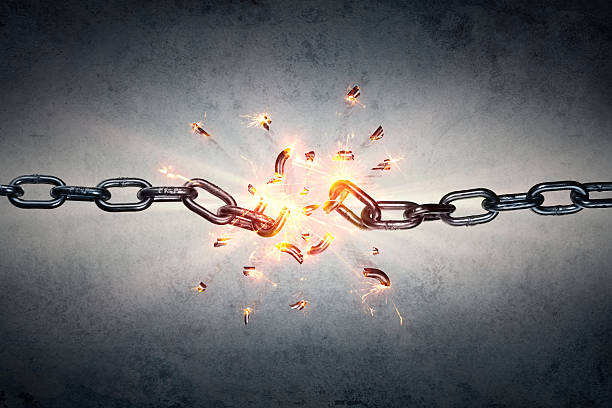
\includegraphics[scale=0.26,keepaspectratio]{Images/Acknowledgements/broken-chain.jpg}
\end{figure}
%

%
%
%% ToC
%
%
\clearpage
\thispagestyle{empty}

\pagestyle{fancy}

\tableofcontents
\clearpage
%
%% Empty page
%
\thispagestyle{empty}
\null
\clearpage

%
%% Start
%
%\pagenumbering{arabic}
\mainmatter

\setcounter{chapter}{-1}
\chapter{Preface}
%
\section{Why Monero?}
I would like to take a moment here and share the experience of selecting a research topic. This was as important to me as the rest of my work. I am not talking about concepts of "good topic" or a list of "factors to consider". I am definitely not an expert on this subject and you can find many valuable information about this process online. I would like to share with you the impact of an argument, about selecting this topic over other options, that was addressed to me by my colleague and friend, Dionysis Zindros. He said to me that in his opinion this topic would be "beneficial for the Monero community".

I strongly recommend before you select your topic of research to take an evening of your time and read a paper titled "The Moral Character of Cryptographic Work", written by Phillip Rogaway~\cite{moral}. No matter how small this world makes you feel, when you select a topic you have responsibility. I was lucky to work with people who understood this and led me to take a moment and think about what cause I really wanted to contribute to.

In our days, cryptographic work is a political action. There is no doubt about that. Think through your intentions and the person you want to be before you select your path. Remember, you have responsibility.
%
\section{An important thank you note}
During my research I had a lot of help from forum answers and conversations and most of all, from the monero stack exchange users~\cite{stackexchange}. I would like to thank many users for their valuable share of knowledge. I had help from a lot of users and several stack exchange forums, who pointed me to the right direction or helped me clarify my misunderstanding of notions from time to time.
\pagebreak

I want to thank them for the aid, but most important, I want to thank everyone who contributes to this knowledge sharing. It means a lot to me and gives me a perspective on my occupation. I don't see the work of a cryptographer as an 8-hour employment to make ends meet. I hope my interests and efforts to be much more than a day job. I feel part of a community that contributes to the real world and keeps me motivated and convinced that our work makes the world a better place to live in. I thank you all for your example.
%
\section{Narrative}
I will change the first person singular narrative. Apart from all the people I have already thanked, my personality has been shaped by my family, my friends, important acquaintances and stories about my heros. All of them are part of me, part of who I am.

As a result, I see this work as a collaboration of all of us and that completes the list of the reasons why I will keep a first person plural narrative from now on. I could not do that in the above paragraphs because this section, as you can understand, is extremely personal. I thank you all.

Another change will be the way I am addressing to you, my reader. It will be, from now on, in a third person point of view. This is just a personal aesthetic choice. I thank you for taking the time to read our work. I hope you find it enjoyable.

\setcounter{chapter}{-1}
\chapter{Introduction}
%
\section{Why Monero?}
\setlength{\intextsep}{0pt}
\begin{wrapfigure}{L}{0.25\textwidth}
\centering

\includegraphics[width=0.25\textwidth]{Images/Introduction/hello.jpg}
\end{wrapfigure}
I would like to take a moment here and share the experience of selecting a research topic. This was as important to me as the rest of my work. I am not talking about concepts of "good topic" or a list of "factors to consider". I am definitely not an expert on this subject and you can find many valuable information about this process online. I would like to share with you the impact of an argument, about selecting this topic over other options, that was addressed to me by my colleague and friend, Dionysis Zindros. He said to me that in his opinion this topic would be "beneficial for the Monero community".

I strongly recommend before you select your topic of research to take an evening of your time and read a paper titled "The Moral Character of Cryptographic Work", written by Phillip Rogaway~\cite{moral}. No matter how small this world makes you feel, when you select a topic you have responsibility. I was lucky to work with people who understood this and led me to take a moment and think about what cause I really wanted to contribute to.

In our days, cryptographic work is a political action. There is no doubt about that. Think through your intentions and the person you want to be before you select your path. Remember, you have responsibility.
%
\section{An important thank you note}
During my research I had a lot of help from forum answers and conversations and most of all, from the monero stack exchange users~\cite{stackexchange}. I would like to thank many users for their valuable share of knowledge. I had help from users \verb|jtgrassie|, \verb|Laxmana|, \verb|knaccc| and a lot more from other stack exchange forums, who pointed me to the right direction or helped me clarify my misunderstanding of notions from time to time.
\pagebreak

I want to thank them for the aid, but most important, I want to thank everyone who contributes to this knowledge sharing. It means a lot to me and gives me a perspective on my occupation. I don't see the work of a cryptographer as an 8-hour employment to make ends meet. I hope my interests and efforts to be much more than a day job. I feel part of a community that contributes to the real world and keeps me motivated and convinced that our work makes the world a better place to live in. I thank you all for your example.
%
\section{Not MY work}
I will change the first person singular narrative because this document is not \textbf{MY} intellectual work. I had a great help from collegues, friends and people all over the world, but most important, this document is a product of who I am. Apart from all the people I have already thanked, my personality has been shaped by my family, my friends, important acquaintances and stories about my heros. All of them are part of me, part of who I am.

As a result, I see this work as a collaboration of all of us and that completes the list of the reasons why I will keep a first person plural narrative from now on. I could not do that in the above paragraphs because this section, as you can understand, is extremely personal. I thank you all.

Another change will be the way I am addressing to you, my reader. It will be, from now on, in a third person point of view. This is just a personal aesthetic choice. I thank you for taking the time to read our work. I hope you find it enjoyable.

\section{Thesis structure}
\setlength{\intextsep}{2pt}
\begin{wrapfigure}{L}{0.2\textwidth}
\centering

\includegraphics[width=0.2\textwidth]{Images/Introduction/structure.png}
\end{wrapfigure}
We tried to make this document readable. From this point of view, we tried to achieve completeness, in the sense that the reader should not refer to external resources to understand the basic arguments involved. Of course, a more keen reader can find references for a detailed study of the notions involved in our work, but that is something that we wanted to be as optional as possible.

In the first chapter, the reader will find an overview of the first complete implementation of a cryptocurrency. That was a paper published under the pseudonym Satoshi Nakamoto~\cite{Nakamoto_bitcoin:a}, introducing the \hyperref[sec:Bitcoin]{Bitcoin} project to the world. This overview is certainly not a detailed description of all aspects of Bitcoin, as this would be unproductive for the discussion in this work. However, we believe that we give a satisfactory description of the project and we hope that the reader will acquire an adequate understanding of the structure of this novelty.

In the second chapter, we introduce the reader to the concept of \hyperref[sec:mining]{mining}, based on the knowledge gained through the study of the first chapter. The purpose of this description is to introduce the notion of \emph{egalitarianism} and more precisely, the notion of \hyperref[sec:egalitarian]{egalitarian mining}. This notion was for a long time a folklore subject of dispute in the community, being a starter for many passionate conversations. It was formally defined recently, in the work of Dimitris Karakostas, Aggelos Kiayias, Christos Nasikas and Dionysis Zindros ~\cite{egalitarianism}.
\pagebreak

In the third chapter we introduce another cryptocurrency, named \hyperref[sec:Monero]{Monero}, and the purposes of its community along with a technical description of its features. The basic structure for Monero project is the \hyperref[sec:CryptoNote]{CryptoNote} protocol, described in a paper published under the pseudonym Nicolas van Saberhagen~\cite{citeulike:14139412}. We describe its features as well.

Then, we get to the point where we can discuss the problem of interest of this thesis. This is Monero's mining function, \hyperref[ch:cryptonight]{CryptoNight}. This function is part of the CryptoNote protocol and it is the reason that Monero claims to offer egalitarianism in its mining process. This feature's existence is due to a known property, called \hyperref[sec:memory-hard]{memory-hardness}. This function is alleged to be memory-hard, although we found no formal research on this matter. CryptoNight's functionality and features are described in chapter four.

In the next chapter, we try to construct a formal mathematical proof of the CryptoNight's memory-hardness property and we discuss the reasons we failed to do so. Using these reasons, we attempt to construct an attack on this property.

Finally, we sum up our observations and try to highlight important knowledge gained through this journey. In the first appendix, the reader can find formal mathematical definitions of the notions used or referred, in an effort for this thesis to be both readable and complete. Constructions and details about the Monero project, can be found in the second Appendix. However, this information is not needed for the reader to keep up with the flow of our work or to understand our remarks. Nevertheless, they were included for the sake of completeness and for the reader, as he/she might find this information beneficial.

\part{From decentralization to re-centralization}

\chapter{Preliminaries}

\epigraph{Security is a binary state. A system cannot be secure against malicious attackers and insecure against other "noble" parties. It is either secure or insecure. And if the prospect of an attack exists, then security collapses.}{\emph{Edward Snowden}}

\section{Cryptography background} \label{ch:math}
%
Here we will include the formal mathematical definition of any cryptographic primitive that the reader will need to study this thesis. Our goal is to make the citation and references in this document an optional read. We believe that we can make this project complete on its own and any available source will be needed only for the experienced reader who may want to get a deeper understanding of the mechanics discused.

A great help, in order to keep this section as concrete as possible, was the work of my collegue and friend Kostis Karantias. He had already defined some notions, which are helpful in this thesis too. Some of his work is reproduced here. I thank him for his help and appreciate his work. I definitely refer the reader to his thesis~\cite{gtklocker}.
%
\subsection{Hash function}
%
We will define the syntax and the security model of the cryptographic hash function, as introduced in \cite{Katz:2007:IMC:1206501}. We will slightly change their definition, because we assume no key as input to the hash function. In our case, the only input is a message.
\clearpage
\pagebreak

\begin{definition}[Hash function - syntax]
A \emph{hash function} is a probabilistic \\
polynomial-time (p.p.t.) algorithm $H$ satisfying the following:
\begin{itemize}
  \item[$\bullet$] There exists a, polynomial in $n$, function $l$ such that $H$ is a (deterministic) p.t. algorithm that takes as input any string $x \in { \{ 0,1 \}}^*$ and outputs a string:
\end{itemize}
\begin{equation} \nonumber
  H(x) \in { \{ 0,1 \}}^{l(n)}
\end{equation}
If for every $n$, $H$ is defined only over inputs of length $l'(n)$ and $l'(n) > l(n)$, then
we say that $H$ is a \emph{fixed-length hash function} with length parameter $l'$. An output of a hash function is called a \emph{digest} of the function.
\end{definition}

Notice that in the fixed-length case we require that $l'$ be greater than $l$. This ensures that the
function is a hash function in the classic sense in that it \emph{compresses} the input. We remark
that in the general case we have no requirement on $l$ because the function takes for input all (finite) binary strings. Thus, by definition, it also compresses.

We will now define security for this model. We begin by defining a game for a hash function $H$, an adversary $\mathcal{A}$ and a security parameter $n$:

\vspace{0.2cm}
\noindent \textbf{The collision-finding game} $\mbox{Hash-coll}_{\mathcal{A},H}(n)$: ~\cite{Katz:2007:IMC:1206501}
\begin{enumerate}
  \item The adversary $\mathcal{A}$ outputs a pair $x$ and $x'$. \\
  Formally, $(x,x') \leftarrow \mathcal{A}(s)$.
  \item The output of the experiment is $1$ if and only if $x \neq x'$ and $H(x) = H(x')$. In such a case, we say that $\mathcal{A}$ has found a collision.
\end{enumerate}
%
The definition of collision resistance for hash functions states that no efficient adversary can find a collision except with negligible probability.
%
\begin{definition}~\textnormal{\cite{Katz:2007:IMC:1206501}}
  A hash function $H$ is \emph{collision resistant} if for all probabilistic polynomial-time adversaries $\mathcal{A}$ there exists a negligible function $\textbf{negl}(\cdot)$ such that

\begin{equation} \label{eqn:collision}
  Pr[\mbox{Hash-coll}_{\mathcal{A},H}(n) = 1] \leq \textbf{negl} \: (n)
\end{equation}
\end{definition}

\subsection{Password Scramblers}
Passwords\footnote{Passphrases and personal identification numbers (PINs) are considered "passwords", in this context.} are user-memorizable secrets. Typical (user-chosen) passwords often suffer from low entropy and can be attacked by trying out all possible password candidates. If we let asside the case of a dedicated cryptographic protocol on an interactive session, the next best protection are password scramblers performing \emph{key-stretching}. Christian Forler, Stefan Lucks and Jakob Wenzel~\cite{ForlerLW13}, give three basic conditions a good password scrambler should satisfy at least:

\begin{enumerate}
  \item \label{Condition 1} Given a password $pwd$, computing $PS(pwd)$ should be "fast enough" for the user.
  \item \label{Condition 2} Computing $PS(pwd)$ should be "as slow as possible", without contradicting \hyperref[Condition 1]{condition}~\ref{Condition 1}.
  \item Given $y=PS(pwd)$, there must be no significantly faster way to test $q$ password candidates $x_1, x_2, \dots, x_q$ for $PS(x_i)=y$ than by actually computing $PS(x_i)$ for each $x_i$.
\end{enumerate}

Tratidionally, most password scramblers satisfy \hyperref[Condition 2]{condition}~\ref{Condition 2} by iterating a cryptographic primitive (a block cipher or hash function) many times. However, an adversary with $b$ computing units (\emph{cores}) can try $b$ different passwords in parallel. With today's availability of graphical processing units (GPUs), slowing down these kind of attacks becomes a pressing question.

\subsection{Memory-Hard Functions} \label{sec:memory-hard}
We will define the notion of the memory-hard function in the Parallel Random Oracle Model (pROM) of \cite{Alwen:2015:HPC:2746539.2746622}, as introduced in \cite{cryptoeprint:2016:875}. First, we will define the model along with the associated complexity notions.

\paragraph{The parallel Random Oracle Model.} We consider an algorithm $\mathcal{A}$ executing in the pROM of \cite{Alwen:2015:HPC:2746539.2746622}. Let this algorithm be repeated an arbitrary amount of times. After each invocation we make states. At invocation $i \in \{ 1,2, \dots \}$ algorithm $\mathcal{A}$ keeps the state $\sigma_{i-1}$ it produced. Next $\mathcal{A}$ can make calls $\textbf{q}_i = (q_{1,i}, q_{2,i}, \dots)$
to the \emph{fixed input length random oracle $H$} (ideal compression function). After it receives the digest of $H$, is allowed to perform arbitrary computation before producing its output (the next state $\sigma_i$). The state $\sigma_0$ contains the input to the computation and no other state is kept by $\mathcal{A}$. Now, we need some complexity notions to be defined.

The cumulative memory complexity (CMC) is defined to be
\begin{equation} \nonumber
    cmc(\mathcal{A}) = \underset{H}{\mathbb{E}} \Bigg{[} \underset{x,r}{\max} \sum_{i} \lvert \sigma_i \rvert \Bigg{]}
\end{equation}
where $\lvert \sigma \rvert$ is the bit-length of state $\sigma$, the expectation is taken over the choice of $H$ and $max_{x,r}$ denotes the maximum over all inputs and coins of $\mathcal{A}$.

Moreover, the \emph{time complexity} (TC), $time(\mathcal{A})$ is the maximum running time of $\mathcal{A}$ in any execution. Similarly, the \emph{space complexity} (SC) is the largest state it ever outputs in any execution.

\paragraph{Oracle function.} Let $f$ be a function over strings depending on the choice of $H$. We consider the scenario in which we want to compute $f$ on $m \in \mathbb{N}^{+}$ arbitrary distinct inputs.
Let $\mathbb{A}_{f,m,q}$ be the set of pROM algorithms that accomplish this, making at most $q$ queries to
$H$. Then,

\begin{enumerate}[label=(\alph*)]
  \item $f$ is an oracle function \\

  \item The \emph{amortized cumulative memory complexity} (aCMC) of $f$ is defined to be
  \begin{equation} \nonumber
      cmc_{m,q}(f) = \min \Bigg{\{} \frac{cmc(\mathcal{A})}{n} : \: n \in [m], \mathcal{A} \in \mathbb{A}_{f,n,q} \Bigg{\}}
  \end{equation}
\end{enumerate}
This definition provides a good lower-bound on the \emph{amortized time complexity} of a function \cite{Alwen:2015:HPC:2746539.2746622}.

For more detailed information about the above, we refer the reader to the appendix of \cite{cryptoeprint:2016:875}. The reader can find some technical details there that are beyond of the scope of this thesis. Now we are ready to define properly the notion of the memory-hard function.


\begin{definition}[Memory-Hard Function] \label{Memhard1}
  Let $\{ f_{\sigma, \tau} \}_{\sigma, \tau \in \mathbb{N}^{+}}$ be a family of (oracle) functions and $\mathcal{N}$ be a sequential pROM algorithm which, on input $(\sigma, \tau, x)$, outputs $f_{\sigma, \tau}(x)$ in time at most $\tau \sigma$ using space at most $\sigma$. Then $F=\big{(} \{ f_{\sigma,\tau} \}, \mathcal{N} \big{)}$
  is an $(h,g,t)$-memory-hard function (for up to $m$ instances and $q$ queries) if it has memory-hardness at least $h(\cdot)$, memory-gap at most $g(\cdot)$ and throughput at least $t(\cdot)$ (all functions of $\sigma$ and $\tau$).

\begin{align*}
cmc_{m,q}(f_{\sigma, \tau})&\geq h(\sigma, \tau)           &  \frac{\mbox{space}(\mathcal{N})*\mbox{time}(\mathcal{N})}{cmc_{m,q}(f_{\sigma, \tau})} &\leq g(\sigma, \tau)             &  \frac{\mbox{space}(\mathcal{N})}{\mbox{time}(\mathcal{N})} &\geq t(\sigma, \tau)\\
\end{align*}
%
\end{definition}

The above definition~\cite{cryptoeprint:2016:875}, although extremely rigid, is not that intuitive. In order to describe memory requirements, we will mention another definition given in \cite{ForlerLW13}, without causing any conflict with the above. Before we give the second definition, one should notice that for any parallelized attack, using $b$ cores, the required memory per core is decreased by a factor of $\frac{1}{b}$, and vice versa.

\begin{definition}[Memory-Hard Function - intuitive]
  Let $g$ denote the memory cost factor. For all $\alpha > 0$, a memory-hard function $f$ can be computed on a Random Access Machine using \textbf{space}$(g)$ space and \textbf{time}$(g)$ operations, where \textbf{space}$(g) \in \Omega(\mbox{\textbf{time}}(g)^{1-\alpha})$.\\

  \noindent Thus, for \textbf{space}$(\cdot)$ \textbf{time}$(\cdot)$\:$=G^2$ with $G=2^g$, using $b$ cores, we have
  \begin{equation} \label{eqn:memhard}
    \Bigg{(} \frac{1}{b} \cdot \mbox{\textbf{space}}(\cdot) \Bigg{)} \bigg{(} b \cdot \mbox{\textbf{time}}(\cdot) \bigg{)} = G^2.
  \end{equation}
\end{definition}
In their paper a formal generalization of this notion is given but it is beyond of the scope of this thesis. For more information about memory-hardness, the reader is refered to their work~\cite{ForlerLW13}.
%
\subsection{Pseudorandom Functions} \label{sec:PRF}
In cryptography, a pseudorandom function family, abbreviated PRF, is a collection of efficiently-computable functions which emulate a random oracle in the following way: no efficient algorithm can distinguish (with significant advantage) between a function chosen randomly from the PRF family and a random oracle (a function whose outputs are fixed completely at random). With that in mind,
we must first recall the definition of oracle indistinguishability and then proceed to define a pseudorandom function. Reproduced from~\cite{ACI}:

\begin{definition}[Oracle Indistinguishability]
  Let $\{ O_n \}_{n \in \mathbb{N}}$ and $\{ O'_{n} \}_{n}$ be ensembles where $O_n, O'_n$ are probability
  distributions over functions $f: \{ 0,1 \}^{l_1(n)} \rightarrow \{ 0,1 \}^{l_2(n)}$ for some polynomials $l_1(\cdot)$, $l_2(\cdot)$. We say that $\{ O_{n} \}_{n}$ and $\{ O'_{n} \}_{n}$ are \emph{computationally indistinguishable} (denoted by $\{ O'_{n} \}_{n} \approx \{ O'_n \}_{n \in \mathbb{N}}$
  ) if for all non-uniform p.p.t. oracles machines $D$, there exists a negligible function $\epsilon(\cdot)$ such that $\forall n \in \mathbb{N}$
  \begin{equation} \label{oracle}
    \Bigg{\lvert} \: Pr \big{[} F \leftarrow O_n : D^{F(\cdot)}(1^n)=1 \big{]} - Pr \big{[} F \leftarrow O'_n : D^{F(\cdot)}(1^n)=1 \big{]} \: \Bigg{\rvert} < \epsilon(n).
  \end{equation}
\end{definition}
\pagebreak

\begin{definition}[Pseudorandom Function]
  A family of functions $\big{\{} f_s: \{ 0,1 \}^{\lvert s \rvert} \rightarrow \{ 0,1 \}^{\lvert s \rvert} \big{\}}_{s \in \{ 0,1 \}^{*}}$ is \emph{pseudorandom} if
  \begin{itemize}
    \item[$\bullet$] (Easy to compute): $f_s(x)$ can be computed by a p.p.t. algorithm that is given input $s$ and $x$
    \item[$\bullet$] (Pseudorandom): $\big{\{} s \leftarrow \{ 0,1 \}^n: f_s \big{\}}_n \approx \big{\{} F \leftarrow RF_n: F \big{\}}_n$.
  \end{itemize}
\end{definition}
\noindent where, $RF_{n}$ is considered a family of functions that are random oracles.

The intuition in this section is that we can't construct a function that actually implements a random oracle. But, for practical purposes, we can construct a function or family of functions that are in distriguishable from random oracles. That is good enough for a security point of view and the next game is necessary in order to define the security model for this mathematical element.
\vspace{0.3cm}
\begin{algorithm}
  \caption{\label{alg:pseudorandom}The \textsf{game} algorithm
    for a pseudorandom function $f_{s}$ (Adversary $\mathcal{A}$)}
    \begin{algorithmic}[1]
      \Function{\sf game$_{\mathcal{A}}^{f_{s}}$}{$n$}
            \State \sf{$b$} $\overset{\$}{\gets}$ \sf{$\{0,1\}$}
              \If{\sf{$b=0$}}
                \State \sf{$f'$} $\gets$ \sf{$\big{\{} \{0,1\}^{n}  \rightarrow \{0,1\}^{n} \big{\}}$}
              \Else
                \State \sf{$f'$} $\gets$ \sf{$f_{s}$}
              \EndIf
              \State \sf{$b^{*}$} $\gets$ \sf{$\mathcal{A}^{f'}(1^{n})$}
              \If{\sf{$b=b^{*}$}}
                \State \Return{1}
              \EndIf
            \State\Return{0}
        \EndFunction
    \end{algorithmic}
\end{algorithm}
\vspace{0.3cm}

\noindent Based on the above algorithm we can now define the security model:

\begin{definition}[Security model]
  Let $f_{s}$ be a pseudorandom function for some $s \in \{0,1\}^{n}$, where $n$ is the security parameter. Then, $\forall$ p.p.t. adversarial algorithm $\mathcal{A}^{f'}$, with access to some random oracle function $f'$, there exists a negligible function $\epsilon(\cdot)$ such that $\forall n \in \mathbb{N}$:

  \begin{equation} \label{eq:secmodel}
    \Bigg{\lvert} \: \underset{s \overset{\$}{\gets} \{0,1\}^{n}}{Pr} \big{[} \mathcal{A}^{f_{s}}(1^{n}) = 0 \big{]} - \underset{f' \overset{\$}{\gets} \big{\{} \{0,1\}^{n}  \rightarrow \{0,1\}^{n} \big{\}}}{Pr} \big{[} \mathcal{A}^{f'}(1^{n}) = 0 \big{]} \: \Bigg{\rvert} < \epsilon(n).
  \end{equation}
\end{definition}

Notice that if someone knows $s$ then it is easy to distinguish $f_s$ from a random function. In order to consider this function indistinguishable from a random function, one should keep seed $s$ secret.
\clearpage
\pagebreak

\subsection{Pebbling game}
Hellman presented in~\cite{Hellman:2006:CTT:2263346.2269686} a possibility to trade memory/space $S$ against time $T$ in attacking cryptographic algorithms, i.e. he has introduced the idea of a time-memory trade-off (TMT) in terms of generic attacks. Hence, we can assume that an adversary with access to this algorithm and restricted resources is always looking for a sweet spot to optimize $S \cdot T$. For, studying the TMT, one needs to choose a certain model. But first we must introduce the reader to the notion of the \emph{directed acyclic graph}. Reproduced from~\cite{ForlerLW13}:

\begin{definition}[Directed Acyclic Graph]
  Let $\Pi(\mathcal{V},\mathcal{E})$ be a graph consisting of a set of vertices $\mathcal{V}=(v_0,v_1,\dots,v_{n-1})$ and a set of edges $\mathcal{E}=(e_0,e_1,\dots,e_{l-1})$, where $\mathcal{E}=\varnothing$ is a valid variant. $\Pi(\mathcal{V},\mathcal{E})$ is a \emph{directed acyclic graph}, if every edge in $\mathcal{E}$
  consists of a starting vertex $v_i$ and an ending vertex $v_j$, with $i \neq j$. A path through $\Pi(\mathcal{V},\mathcal{E})$ beginning at vertex $v_i$ must never reach $v_i$ again (else, there would be a cycle). If there exists a path from a vertex $v_i$ to a vertex $v_j$ in the graph with $i \neq j$, we will write $v_i \leq v_j$.
\end{definition}

In 1970, Hewitt and Paterson introduced a method for analyzing TMTs on directed acyclic graphs (DAG), called \emph{pebbling game}. It has been occasionally used in cryptographic context, see e.g.~\cite{Dziembowski:2011:KSR:2033036.2033061} for a recent example. The pebble game model is restricted to DAGs with bounded in-degree and can be seen as a single-player game. The two following definitions are produced from~\cite{cryptoeprint:2016:875}:

\begin{definition}[Parallel/Sequential Graph Pebbling]
  Let $G=(\mathcal{V},\mathcal{E})$ be a DAG and let $T \subseteq \mathcal{V}$ be a target set of nodes to be pebbled. A pebbling configuration (of $G$) is a subset $P_i \subseteq \mathcal{V}$. A legal parallel pebbling of $T$ is a sequence $P=(P_0,\dots,P_t)$ of pebbling configurations of $G$ where $P_0 = \varnothing$ and which satisfies \hyperref[pebble:condition_1]{conditions}~\ref{pebble:condition_1}
  \hyperref[pebble:condition_2]{\&}~\ref{pebble:condition_2} below. A sequential pebbling additionally must satisfy \hyperref[pebble:condition_3]{condition}~\ref{pebble:condition_3}.

  \begin{enumerate}
    \item \label{pebble:condition_1} At some step every target node is pebbled (though not necessarily simultaneously).
%
    \begin{equation} \label{eqn:pebcondition_1}
      \forall x \in T \ \ \exists z \leq t \quad : \quad x \in P_z.
    \end{equation}
%
    \item \label{pebble:condition_2} Pebbles are added only when their predecessors already have a pebble at the end of the previous step.
%
    \begin{equation} \label{eqn:pebcondition_2}
      \forall i \in [t] \quad : \quad x \in (P_i \setminus P_{i-1}) \ \Rightarrow \ \mbox{\textbf{parents}}(x) \subseteq P_{i-1}.
    \end{equation}
%
    \item \label{pebble:condition_3} At most one pebble placed per step.
%
    \begin{equation} \label{eqn:pebcondition_3}
      \forall i \in [t] \quad : \quad \lvert P_i \setminus P_{i-1} \rvert \leq 1.
    \end{equation}
%
  \end{enumerate}
%
  We denote with $\mathcal{P}_{G,T}$ and $\mathcal{P}_{G,T}^{||}$ the set of all legal sequential and parallel pebblings of $G$ with target set $T$, respectively.
  Note that $\mathcal{P}_{G,T} \subseteq \mathcal{P}_{G,T}^{||}$. In the case where $T=\mbox{\textbf{sinks}}(G)$, we will simply write $\mathcal{P}_{G}$ and
  $\mathcal{P}_{G}^{||}$.
%
\end{definition}
%
\begin{definition}[Time/Space/Cumulative Pebbling Complexity]
  The \emph{time}, \emph{space}, \emph{space-time} and \emph{cumulative} complexity of a pebbling $P=\{ P_0,\dots,P_t \} \in \mathcal{P}_{G}^{||}$ are defined to be:

  \begin{align*}
    \Pi_t(P)&= t  &  \Pi_s(P)&= \underset{i \in [t]}{\max} \lvert P_i \rvert &  \Pi_{st}(P)&= \Pi_t(P) \cdot \Pi_s(P) & \Pi_{cc}(P)&= \underset{i \in [t]}{\sum} \lvert P_i \rvert .\\
  \end{align*}
  For $\alpha \in \{ s,t,st,cc \}$ and a target set $T \subseteq \mathcal{V}$, the \emph{sequential} and \emph{parallel} pebbling complexities of $G$ are defined as

  \begin{align*}
    \Pi_\alpha(G,T)&= \underset{P \in \mathcal{P}_{G,T}}{\min} \Pi_{\alpha}(P) &  &\mbox{and} & \Pi_{\alpha}^{||}(G,T)&= \underset{P \in \mathcal{P}_{G,T}^{||}}{\min} \Pi_{\alpha}(P) .\\
  \end{align*}
  When $T=\mbox{\textbf{sinks}}(G)$, we simplify notation and write $\Pi_{\alpha}(G)$ and $\Pi_{\alpha}^{||}(G)$.
%
\end{definition}
We notice that the definition comes along with the intuition about these complexities. For $\alpha \in \{ s,t,st,cc \}$ and any $G$, the parallel pebbling complexity is at most as high as the sequential,
i.e., $\Pi_\alpha(G) \geq \Pi_{\alpha}^{||}(G)$, and cumulative complexity is at most as high as space-time complexity, i.e. $\Pi_{st}(G) \geq \Pi_{cc}(G)$ and $\Pi_{st}^{||}(G) \geq \Pi_{cc}^{||}(G)$.
\clearpage
\pagebreak

\section{Bitcoin} \label{sec:Bitcoin}
Bitcoin~\cite{Nakamoto_bitcoin:a} is a decentralized digital currency that enables instant payments to anyone, anywhere in the world. Bitcoin uses peer-to-peer technology to operate with no central authority: transaction management and money issuance are carried out collectively by the network.

The original Bitcoin software by Satoshi Nakamoto was released under the MIT license. Most client software, derived or "from scratch", also use open source licensing.

Bitcoin is the first successful implementation of a distributed cryptocurrency, described in part in 1998 by Wei Dai on the cypherpunks mailing list. For the reader to understand what this list was, we reproduce from \emph{cryptoanarchy.wiki}~\cite{cryptoanarchy}:

\begin{verbatim}
  The Cypherpunks mailing list was started in 1992, and by 1994
  had 700 subscribers. At its peak, it was a very active forum
  with technical discussion ranging over mathematics, cryptography,
  computer science, political and philosophical discussion,
  personal arguments and attacks, etc., with some spam thrown in.
  An email from John Gilmore reports an average of 30 messages
  a day from December 1, 1996 to March 1, 1999, and suggests that
  the number was probably higher earlier. The number of subscribers
  is estimated to have reached 2000 in the year 1997.
\end{verbatim}

It is during this period that the community was energised by a battle with the U.S. intelligence establishment relating to the export of cryptography (which the U.S. Government had at the time classified as a munition).

This is a battle that the cypherpunk movement and broader civilian cryptography community largely won, though some variations of government proposals still pop up to this day. More about the cypherpunks mailing list and the archived conversations can be found in cryptoanarchy wiki~\cite{cryptoanarchy}.

Building upon the notion that money is any object, or any sort of record, accepted as payment for goods and services and repayment of debts in a given country or socio-economic context, Bitcoin is designed around the idea of using cryptography to control the creation and transfer of money rather than relying on central authorities.

Bitcoin is pseudonymous~\cite{gtklocker}: the identity of each user is only their \emph{address} (a user can have multiple addresses), which corresponds to an ECDSA public key~\cite{ecdsa}. This address can be used to receive money from other users. Each user can spend money only if they have their corresponding private key. A set of ECDSA keypairs comprises a \emph{wallet}.

As in fiat money, transfer of value in Bitcoin happens with transactions. A \hyperref[sec:transactions]{transaction} has \hyperref[sec:inputs]{inputs} and \hyperref[sec:outputs]{outputs} (see \hyperref[sec:outputs]{sections}~\ref{sec:transactions},~\ref{sec:inputs},~\ref{sec:outputs}). An output is where the value creation happens for the receiver. An output can be later redeemed by using its designated receiver's private key and turned into an input to be used for another transaction.

Bitcoins have all the desirable properties of a money-like good. They are portable, durable, divisible, recognizable, fungible, scarce and difficult to counterfeit.
\pagebreak

\subsection{Transactions} \label{sec:transactions}
A \emph{transaction} is a collection of inputs and outputs. It uses the sum of the inputs' values as credit to debit each output accordingly. As it makes sense, a transaction is only valid as long as all its outputs and inputs are valid. It should also be clear that the value of the outputs should not exceed the value of the inputs, otherwise we would be creating value out of thin air with new transactions. Specifically this is expressed as

\begin{equation} \nonumber
  \sum_{\sf i \in inputs} {\sf i.value} \ge \sum_{\sf o \in outputs} {\sf o.value}
\end{equation}

This is sometimes called the \emph{Law of Conservation}. In cases where

\begin{equation} \nonumber
  \sum_{\sf i \in inputs} {\sf i.value} > \sum_{\sf o \in outputs} {\sf o.value}
\end{equation}
we call
\begin{equation} \nonumber
  \sum_{\sf i \in inputs} {\sf i.value} - \sum_{\sf o \in outputs} {\sf o.value}
\end{equation}
the \emph{transaction fee}.

The transaction id is the digest of the two times hashing operation (SHA256\textsuperscript{2}) on the transaction data. In \hyperref[fig:transaction-internally]{figure}~\ref{fig:transaction-internally} the reader can see the notion described above in practice.

\vspace{0.3cm}
\begin{figure}[ht]
  \centering
  \includegraphics[width=1.1\columnwidth,keepaspectratio]{Images/transaction-internally.png}
  \caption{Transactions with their inputs and outputs~\cite{mastering}}
  \label{fig:transaction-internally}
\end{figure}
\pagebreak

\subsection{Inputs} \label{sec:inputs}
An input is the way an output is redeemed. Specifically, it contains three things:
\begin{itemize}
  \item The hash of the transaction where the output of interest is contained.
  \item An index clarifying which output in the transaction this input is referring to.
  \item A signature used for the validation of the output script.
\end{itemize}

As a convention, when we talk about the value of an input we mean the value of the output it redeems.

\subsection{Outputs} \label{sec:outputs}
An \emph{output} is a tuple ({\sf value, pubKeyScript}). The \textsf{value} refers to an amount of Bitcoin in Satoshi (where $\sf 10^8 \, Satoshi = 1 \, \bitcoin$) and \textsf{pubKeyScript} is a boolean check in order for \textsf{value} to be transferable (see \hyperref[sec:scripts]{section}~\ref{sec:scripts}).

\subsection{Blocks} \label{sec:blocks}
A block is a collection of transactions. A valid block satisfies the following:

\begin{itemize}
  \item there are no double spends (all the inputs are unique)
  \item Each transaction is included once
\end{itemize}
The block id is the digest (SHA256) of the block data.

\vspace{0.3cm}
\begin{figure}[bh]
  \centering
  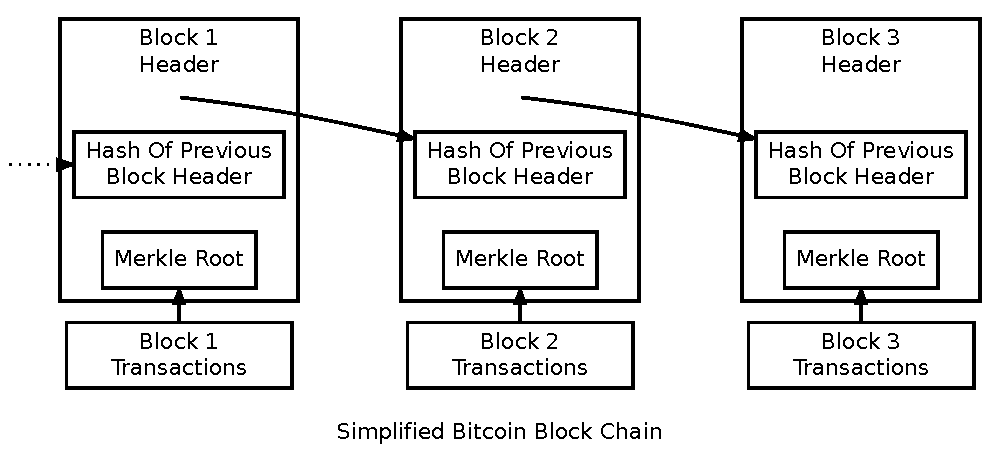
\includegraphics[width=\columnwidth,keepaspectratio]{Images/block-structure.pdf}
  \caption{The block structure~\cite{Nakamoto_bitcoin:a}}
  \label{fig:block-structure}
\end{figure}
\vspace{0.3cm}

A block header contains mainly the hash of the previous block, a \hyperref[sec:merkle-trees]{Merkle root hash} (see \hyperref[sec:merkle-trees]{section}~\ref{sec:merkle-trees}) to commit to a set of transactions, and a nonce. Blocks are always referenced by the hash of their block header. Once a transaction has been included in a valid block it's called \emph{confirmed}.

\subsection{Merkle Trees} \label{sec:merkle-trees}
In this section we will describe a data structure needed by the meticulous reader in order to understand the description of the \hyperref[sec:Bitcoin]{Bitcoin} protocol (see \hyperref[sec:Bitcoin]{chapter}~\ref{sec:Bitcoin}).
A Merkle tree~\cite{merkle} is a data structure which allows a party to commit to a set of items using only a single hash and prove the inclusion of any item in the committed set, by providing a logarithmic proof in terms of the cardinality of the set.

More specifically, the hashes of the items consist the leaves of the tree and the last level. The internal levels are defined recursively as follows: To create level $k-1$ each pair of level $k$, $(A, B)$, is transformed as a node of value $H(A || B)$ which points to both $A$ and $B$ for some hash function $H(\cdot)$. If the number of nodes at level $k$ is odd, the last node at that level is paired with itself\footnote{This specific construction is the one Bitcoin implements. There are various other constructions which are beyond the scope of our work.}.

\begin{figure}[ht]
  \centering
  \includegraphics[width=\columnwidth,keepaspectratio]{Images/merkle-tree-proof.png}
  \caption{A Bitcoin Merkle tree. Source:~\cite{mastering}}
  \label{fig:merkletree}
\end{figure}

Merkle trees are useful in Bitcoin in order to commit to a set of transactions that will be included in a block while keeping the block header of a constant size.

To provide proof of inclusion, all a prover has to do is provide a path of siblings up to the root $\sf{siblings}$ and a bit vector $\sf{left}$ indicating whether each sibling is on the left or the right. The verification process is shown in \hyperref[alg:merkle-verification]{Algorithm}~\ref{alg:merkle-verification}~\cite{gtklocker}.

\begin{algorithm}
  \caption{\label{alg:merkle-verification}The \textsf{Verify} algorithm
    for a Merkle proof}
    \begin{algorithmic}[1]
      \Function{\sf Verify$_{\sf root}$}{\sf leaf, siblings, left}
            \State \sf{currentHash} $\gets$ \sf{leaf}
            \While{$\sf{left} \neq []$}
              \State \sf{siblingIsLeft} $\gets$ \sf{left.shift()}
              \If{\sf{siblingIsLeft}}
                \State \sf{currentHash} $\gets$ \sf{H(siblings.shift() || currentHash)}
              \Else
                \State \sf{currentHash} $\gets$ \sf{H(currentHash || siblings.shift())}
              \EndIf
            \EndWhile
            \State\Return{currentHash = root}
        \EndFunction
    \end{algorithmic}
\end{algorithm}

%An example of a Bitcoin Merkle tree, along with a proof of inclusion for $K$ can be seen on \hyperref[fig:merkletree]{figure}~\ref{fig:merkletree}.

\subsection{Blockchain} \label{sec:blockchain}
Each block contains a SHA-256 cryptographic hash of the previous block~\cite{economist}, thus linking it to the previous block and giving the blockchain its name. Now, the reader can visualize the famous term \emph{blockchain}. The blockchain is a chain of blocks. The blockchain is public and it holds the history of all valid transactions in a cryptocurrency's network. It holds the timeline of a cryptocurrency's life. It is easy to see that, by the definition of the blockchain, there can be no parallel chains. There is not such thing in economics as two valid transaction histories.

It's possible that there are contending chains of blocks. We then say, there is a \emph{fork} on the chain. On \hyperref[fig:blocks]{figure}~\ref{fig:blocks}, the chain has forked on blocks 3 and 6.

We call any valid blocks which are not part of our active chain \emph{orphans}. In our example blocks 4b, 7a and 8a are orphans. As expected, orphan blocks, although typically valid, cannot be part of the transaction history. So, transactions that are included in an orphan block (and have not been included in another block yet) return back in the pool (become \emph{unconfirmed}\footnote{Note: The reader may find this peculiar. However, we observe that as the blockchain grows, older blocks become "safer" (less probability to become orphans). That means that after a transaction becomes confirmed (included in a valid block), one should wait until this valid block is "safe enough".}) and are expected to be included in a block in the future.

\vspace{0.3cm}
\begin{figure}[H]
  \centering
  \includegraphics[width=\columnwidth,keepaspectratio]{Images/blocks.png}
  \caption{A blockchain (the orange blocks are orphans)~\cite{mastering}}
  \label{fig:blocks}
\end{figure}

\subsection{Mining}
We need to maintain a chronological sequence of transactions. In order to avoid several types of attacks we need everyone to agree in some common transaction history. This agreement is called \emph{consensus}. Mining\footnote{It is misleading to think that there is an analogy between gold mining and cryptocurrency mining. The fact is that gold miners are rewarded for producing gold, while some cryptocurrency's miners are not rewarded for producing cryptocoins; they are rewarded for their record-keeping services.} is the processing of transactions in the digital currency system, in which the records of some cryptocurrency's current  transactions, \hyperref[sec:blocks]{\emph{blocks}} (see \hyperref[sec:blocks]{section}~\ref{sec:blocks}), are added to the record of past transactions, the \hyperref[sec:blockchain]{\emph{blockchain}} (see \hyperref[sec:blockchain]{section}~\ref{sec:blockchain}). Miners keep the blockchain consistent, complete, and unalterable by repeatedly grouping newly broadcast transactions into a block, which is then broadcast to the network and verified by recipient nodes~\cite{economist}.

A block contains a list of transactions, the first of which is called the \emph{coinbase transaction} which is where value creation happens in Bitcoin. The miner crafts this transaction granting them some amount of Bitcoins and this transaction is going to be valid only if the block turns out valid. The amount of the \emph{coinbase transaction} is fixed by the Bitcoin protocol. This is a way Bitcoin uses to incentivize miners. However, this doesn't mean that anyone can generate Bitcoin out of thin air: we'll see shortly how it actually comes at a cost with \hyperref[sec:proofofwork]{Proof of Work (PoW)} (see \hyperref[sec:proofofwork]{section}~\ref{sec:proofofwork}).

\subsection{Proof of Work (PoW)} \label{sec:proofofwork}
The key to making Bitcoin decentralized is a technique called Proof of Work (PoW). Proof of Work was first invented in 1992 by Dwork et al.~\cite{dwork} as a measure of limiting email spam and denial of service attacks and later explored by Back~\cite{hashcash} as Hashcash.

We'll examine a simplified model of Hashcash in order to explore the idea. Suppose we want to send an email to someone. In order to prove we've done work, we include a header (like \code{X-Hashcash}), which includes the receiver's email address, and a nonce\footnote{Hashcash headers actually contain 7 different fields which have been omitted here for simplicity. The simplified version explained here is not making the same security guarantees as Hashcash.}. The nonce is picked so that the hash of the header $H(email || nonce)$ has its 20 most significant bits be all 0. The only feasible way to find this is by brute-forcing the nonce. Once the sender has found the nonce, it's included in the header and sent.

The receiver can then very easily check whether the header hashes to a valid value. If that's so, the email it contains belongs to the receiver and the header is not being reused. After this confirmation, the email can be considered not spam.

To reiterate, the idea is having a series of data to commit to and a hole for the nonce, which is brute-forced to satisfy a necessary predicate on the hash, specifically that its $n$ most significant bits are all zeroes. This is exactly how Bitcoin implements Proof of Work. Instead of the hole being on an email header the hole is on the block header. For a block to be valid, its header has to satisfy a predicate like the above.

Bitcoin introduces a couple of differences. $n$ varies according to the block generation rate. Specifically, to translate the previous predicate to Bitcoin terminology, the hash of each block header has to satisfy
\begin{equation} \label{eq:PoW}
  H({\sf blockHeader}) \le T
\end{equation}
where $T$ is called the \emph{target}. As the target goes up, the probability of being below it goes up and generating a valid block is easier. Conversely, if the target goes down it's harder to generate a valid block. To express this, in Bitcoin, the value $\frac{1}{T}$ is called the \emph{difficulty}.

To account for the block generation rate, which Bitcoin tries to keep to 1 block per 10 minutes, every 2016 blocks the target (and subsequently the difficulty) is adjusted accordingly. The target is calculated inside the Bitcoin software and is only a function of the blocks previously seen (frequently called their \emph{view}). So, as long as the Bitcoin nodes agree on the view, they'll agree on the target and all will consider the same set of incoming blocks as valid.

\subsection{Simplified Payment Verification (SPV)}
The size of the blockchain has reached 197GB by the beggining of January 2019, which makes it a very time consuming or even infeasible process to synchronise a full node. Fortunately, a solution was proposed in the original white paper ~\cite{Nakamoto_bitcoin:a}, which allows the creation of so-called \emph{lite nodes}.

Lite nodes only know the headers of the entire blockchain, which are constant-size for each block (80 bytes). At the time of writing of this thesis, the size of all block headers was $\sim$45MB. The lite node then asks the network for transactions concerning it (e.g. transactions concerning a specific public key). Full nodes of the network find such transactions and return them to the requester. For each transaction, the block header of the block it is included in, is returned along with a \hyperref[sec:merkle-trees]{Merkle tree} (see \hyperref[sec:merkle-trees]{section}~\ref{sec:merkle-trees}) proof of inclusion which the lite node can then verify.

This protocol is reliable, as long as an adversary does not control the network of a lite node.

\subsection{Smart contracts}
The idea of the smart contracts was first proposed by Nick Szabo~\cite{szabo}. The proposal was about a computerized transaction protocol that executes the terms of a contract. A set of promises, specified in digital form, including protocols within which the parties perform on these promises. On blockchain, this idea can expand in a general purpose computation.

The reader may be familiar with the notion of smart contracts because of the popular implementation in Ethereum blockchain. However, we should note here that the original smart contract language is Bitcoin!

In the next section we will analyze the basic use of the Bitcoin Scripts.

\subsection{Scripts} \label{sec:scripts}
Bitcoin offers much more than just moving currency around. It allows us to actually move currency conditionally, where the condition can be expressed as a \emph{Bitcoin script}. Bitcoin script is a stack-based language. An example of a Bitcoin script can be seen on \hyperref[fig:bitcoin-script]{figure}~\ref{fig:bitcoin-script}.

\vspace{0.3cm}
\begin{figure}[hb]
  \centering
  {
    \tt
    OP\_HASH256 \\
    6fe28c0ab6f1b372c1a6a246ae63f74f931e8365e15a089c68d6190000000000 \\
    OP\_EQUAL
  }
  \caption{A Bitcoin script~\cite{gtklocker}}
  \label{fig:bitcoin-script}
\end{figure}
\vspace{0.3cm}

This script introduces two kinds of formats. The first kind is commands prefixed with \code{OP\_}. These operations are called \emph{opcodes} and they perform calculations on values on the stack. The result is pushed again to the stack. The types of the calculations are intuitive, e.g. \code{OP\_HASH256} calculates the SHA256 hash of the value on the top of the stack, \code{OP\_EQUALS} compares the top 2 values on the stack and pushes 1 if they are indeed equal or 0 otherwise. The second kind is hex values. These values are simply pushed to the stack. Usually they will be used as input for some operation.

It is easy for the reader to see that the script of \hyperref[fig:bitcoin-script]{figure}~\ref{fig:bitcoin-script} checks if the value on the stack is the preimage of the given hash value and returns 1 (true) or 0 (false). More information about Bitcoin scripts and details about the stack operations can be found in~\cite{wiki}. In practice, this output confirms the success of the evaluation. Such a script is called a \textsf{pubKeyScript}. However, in our example we assume the preimage was on the stack. The way this is implemented in Bitcoin is running another script called \textsf{scriptSig} that passes the parameters to \textsf{pubKeyScript}. The combination of these two scripts is enough powerful and the calculations they perform can be used to make a transaction in the Bitcoin network.
\clearpage
\pagebreak

\subsection{P2PKH}
Now, let's see the standard script for conventional fund transfer in Bitcoin, called \emph{pay to public key hash} (P2PKH). Two types of payment are referred as P2PK (pay to public key) and P2PKH (pay to public key hash). Satoshi later decided to use P2PKH instead of P2PK for two reasons:

\begin{itemize}
  \item Elliptic Curve Cryptography is vulnerable to a modified Shor's algorithm for solving the discrete logarithm problem on elliptic curves. That means, that in the future a quantum computer might be able to retrieve a private key from a public key. By publishing the public key only when coins are spent (and assuming that addresses are not reused), such an attack is rendered ineffective.
  \item With the hash being smaller (20 bytes) it is easier to print and easier to embed into small storage mediums like QR codes.
\end{itemize}

A Bitcoin address is only a hash, so the sender can't provide a full public key in \textsf{pubKeyScript}. When redeeming coins that have been sent to a Bitcoin address, the recipient provides both the signature and the public key. The script verifies that the provided public key does hash to the hash in \textsf{pubKeyScript}, and then it also checks the signature against the public key. The reader can see the process in detail in \hyperref[tab:bitcoin]{table}~\ref{tab:bitcoin}.

\begin{table}[ht]
  \centering
\begin{tabular}{@{}lll@{}}
\toprule
\rowcolor[HTML]{C0C0C0}
\multicolumn{1}{c}{\cellcolor[HTML]{C0C0C0}\textbf{Stack}}                                                                                                                                          & \multicolumn{1}{c}{\cellcolor[HTML]{C0C0C0}\textbf{Script}}                                                                                                                                                          & \multicolumn{1}{c}{\cellcolor[HTML]{C0C0C0}\textbf{Description}}                                                   \\ \midrule
\multicolumn{1}{|l|}{Empty}                                                                                                                                                                         & \multicolumn{1}{l|}{\begin{tabular}[c]{@{}l@{}}\textless{}sig\textgreater{}\textless{}pubKey\textgreater \\ OP\_DUP OP\_HASH160\\ \textless{}pubKeyHash\textgreater \\ OP\_EQUALVERIFY \\ OP\_CHECKSIG\end{tabular}} & \multicolumn{1}{l|}{\begin{tabular}[c]{@{}l@{}}scriptSig and\\ scriptPubKey\end{tabular}}                          \\ \midrule
\multicolumn{1}{|l|}{\begin{tabular}[c]{@{}l@{}}\textless{}pubKey\textgreater\\ \textless{}sig\textgreater{}\end{tabular}}                                                                          & \multicolumn{1}{l|}{\begin{tabular}[c]{@{}l@{}}OP\_DUP OP\_HASH160\\ \textless{}pubKeyHash\textgreater \\ OP\_EQUALVERIFY \\ OP\_CHECKSIG\end{tabular}}                                                              & \multicolumn{1}{l|}{\cellcolor[HTML]{FFFFFF}\begin{tabular}[c]{@{}l@{}}Constants\\ added\\ to stack.\end{tabular}} \\ \midrule
\multicolumn{1}{|l|}{\begin{tabular}[c]{@{}l@{}}\textless{}pubKey\textgreater\\ \textless{}pubKey\textgreater\\ \textless{}sig\textgreater{}\end{tabular}}                                          & \multicolumn{1}{l|}{\begin{tabular}[c]{@{}l@{}}OP\_HASH160\\ \textless{}pubKeyHash\textgreater \\ OP\_EQUALVERIFY \\ OP\_CHECKSIG\end{tabular}}                                                                      & \multicolumn{1}{l|}{\begin{tabular}[c]{@{}l@{}}Top stack\\ item\\ duplicated.\end{tabular}}                        \\ \midrule
\multicolumn{1}{|l|}{\begin{tabular}[c]{@{}l@{}}\textless{}pubKeyHashA\textgreater\\ \textless{}pubKey\textgreater\\ \textless{}sig\textgreater{}\end{tabular}}                                     & \multicolumn{1}{l|}{\begin{tabular}[c]{@{}l@{}}\textless{}pubKeyHash\textgreater \\ OP\_EQUALVERIFY \\ OP\_CHECKSIG\end{tabular}}                                                                                    & \multicolumn{1}{l|}{\begin{tabular}[c]{@{}l@{}}Top stack\\ item\\ hashed.\end{tabular}}                            \\ \midrule
\multicolumn{1}{|l|}{\begin{tabular}[c]{@{}l@{}}\textless{}pubKeyHash\textgreater\\ \textless{}pubKeyHashA\textgreater\\ \textless{}pubKey\textgreater\\ \textless{}sig\textgreater{}\end{tabular}} & \multicolumn{1}{l|}{\begin{tabular}[c]{@{}l@{}}OP\_EQUALVERIFY \\ OP\_CHECKSIG\end{tabular}}                                                                                                                         & \multicolumn{1}{l|}{\begin{tabular}[c]{@{}l@{}}Constant\\ added.\end{tabular}}                                     \\ \midrule
\multicolumn{1}{|l|}{\begin{tabular}[c]{@{}l@{}}\textless{}pubKey\textgreater\\ \textless{}sig\textgreater{}\end{tabular}}                                                                          & \multicolumn{1}{l|}{OP\_CHECKSIG}                                                                                                                                                                                    & \multicolumn{1}{l|}{\begin{tabular}[c]{@{}l@{}}Equality check\\ between the\\ top two stack\\ items.\end{tabular}} \\ \midrule
True                                                                                                                                                                                                & Empty.                                                                                                                                                                                                               & \begin{tabular}[c]{@{}l@{}}Signature is\\ checked for top\\ two stack items.\end{tabular}                          \\ \bottomrule
\end{tabular}
\bigskip
\caption{Bitcoin script process (successful)~\cite{wiki}}
\label{tab:bitcoin}
\end{table}

This is the standard script for conventional fund transfer in Bitcoin. Let's say we want to make sure only Bob can satisfy this script. The \textsf{pubKeyScript} is the following:
\begin{center}
  \code{OP\_DUP OP\_HASH160 <Bob's address> OP\_EQUALVERIFY\footnote{This operation is a lot like \code{OP\_EQUAL} but instead of pushing 1 or 0  to the stack, it fails the script if the arguments are not equal or does nothing otherwise.} OP\_CHECKSIG}
\end{center}
\noindent The \textsf{scriptSig} is then typically \code{<Bob's signature> <Bob's public key>}.

Bob's signature will be available. We will see that it can be found on the hash of the transaction containing the output. The script will then duplicate his public key, check that it matches the one on the \text{pubKeyScript} and if it does, it will check that he has provided a valid signature with that public key. If all these checks pass, the stack will end up with 1 on top and the execution will be valid.


%%%%%%%%%%%%%%%%%%%%%%%%%%%%%%%%%%%%%%%%%%%%%%%%%%%%%%%%%%%%%%%%%%%%%%%%%%%%%%%%
%%%%%%%%%%%%%%%%%%%%%%%%%%%%%%%%%%%%%%%%%%%%%%%%%%%%%%%%%%%%%%%%%%%%%%%%%%%%%%%%
%%%%%%%%%%%%%%%%%%%%%%%%%%%%%%%%%%%%%%%%%%%%%%%%%%%%%%%%%%%%%%%%%%%%%%%%%%%%%%%%
\clearpage
\pagebreak

\section{Egalitarian Mining} \label{sec:mining}


To be accepted by the rest of the network, a new block must contain a \hyperref[sec:proofofwork]{Proof of Work (PoW)} (see \hyperref[sec:proofofwork]{section}~\ref{sec:proofofwork}). The PoW requires miners to find a number called a nonce, such that when the block content is hashed along with the nonce, the result is numerically smaller than the network's difficulty target~\cite{Nakamoto_bitcoin:a} and thus the \hyperref[eq:PoW]{PoW equation} (see \hyperref[eq:PoW]{equation}~\ref{eq:PoW}) is satisfied. This proof is easy for any node in the network to verify, but extremely time-consuming to generate, as for a secure cryptographic hash, miners must try many different nonce values before meeting the difficulty target.

The primary purpose of mining is to set the history of transactions in a way that is computationally impractical to modify by any one entity. By downloading and verifying the blockchain, nodes are able to reach consensus about the ordering of events in some proof of work cryptocurrency~\cite{wiki}.

As we noted in \hyperref[sec:proofofwork]{section}~\ref{sec:proofofwork}, every 2,016 blocks the difficulty target is adjusted based on the network's recent performance, with the aim of keeping the average time between new blocks at ten minutes. In this way, the system automatically adapts to the total amount of mining power on the network. Between 1 March 2014 and 1 March 2015, the average number of nonces, miners had to try before creating a new block, increased from 16.4 quintillion to 200.5 quintillion~\cite{difficulty_history}.

The proof of work system, alongside the chaining of blocks, makes modifications of the blockchain extremely hard, as an attacker must modify all subsequent blocks in order for the modifications of one block to be accepted. As new blocks are mined all the time, the difficulty of modifying a block increases as time passes and the number of subsequent blocks (also called confirmations of the given block) increases~\cite{economist}.

Mining is also the mechanism used to introduce coins into the system: Miners are paid any transaction fees as well as a "subsidy" of newly created cryptocoins. This both serves the purpose of disseminating new cryptocoins in a decentralized manner as well as motivating people to provide security for the system~\cite{wiki}. To elaborate on the second part of this purpose, one can think about the structure of the consensus on the network. The network agrees by majority. So an attacker who controls 51\% of the mining power can successfully attack this structure. As more honest miners contribute to the network, the 51\% attack becomes less feasible.

\begin{wrapfigure}{R}{0.52\textwidth}
  \centering
  \includegraphics[width=0.52\textwidth,keepaspectratio]{Images/Bitcoin/mining.jpeg}
  \caption{Mining options}
  \label{fig:mining}
\end{wrapfigure}
Originally, Bitcoin mining was conducted on the CPUs of individual computers, with more cores and greater speed resulting in more profitability. After that, the system became dominated by multi-graphics card systems, then field-programmable gate arrays (FPGAs) and finally application-specific integrated circuits (ASICs), in the attempt to find more hashes per hour with less electrical power usage (see \hyperref[fig:mining]{figure}~\ref{fig:mining}).

Due to this constant escalation, it has become hard for prospective new miners to start. This adjustable difficulty is an intentional mechanism created to prevent inflation. To get around that problem, individuals often work in \emph{mining pools}. Mining pools are groups of miners who join their collective computational power and share their profit according to the contribution of each party.

Bitcoin generally started with individuals and small organizations handling the mining. At that time, start-up could be enabled by a single high-end gaming system. However, nowadays larger mining organizations might spend tens of thousands on one high-performance, specialized, application-specific integrated circuit.

That creates a problem. In a system, which since its creation is supposed to distribute power among users, there has been a great power concentration in the hands of big companies, like Bitfury or 21, that develop ASICs to mine Bitcoin. Because of the extreme cost of ASICs and extreme hashrate, someone who uses a multi-graphics card system or a CPU is out of competition. As a result, independent miners have largely dried up.

\subsection{Egalitarianism} \label{sec:egalitarian}
\setlength{\intextsep}{0pt}
\begin{wrapfigure}[7]{L}{0.32\textwidth}
\centering

\includegraphics[width=0.32\textwidth]{Images/Mining/justice.jpg}
\end{wrapfigure}
Let's consider several contexts where an adversary has an upper hand over the defender, by using special hardware in an attack. These include password processing, hard-drive protection, cryptocurrency mining, resourse sharing, code obfuscation, etc. \hyperref[sec:memory-hard]{Memory-hard} computing is a generic paradigm, which can protect the defender against attacks in the aforementioned contexts. Every task is amalgamated with a certain procedure requiring intensive access to RAM, both in terms of size and bandwidth, so that transferring the computation to GPU, FPGA, and even ASIC brings little to no cost reduction.

Cryptographic schemes that run in this framework become \emph{egalitarian} in the sense that both users and attackers are equal in the price-performance ratio conditions. When the cryptographic scheme is a hash function used for cryptocurrency mining, we refer to this notion as \emph{egalitarian mining}.

But let's step back a little and think about the need for such a notion. Do we actually need it? Is egalitarian mining a way to destroy competition? Is it unfair? Shouldn't a miner be rewarded for the extra money he invested?

Many questions like the above have been asked and usually the answer is not descriptive enough of what really memory-hardness introduces to the world. We will try here to demonstrate concretely what it means for a cryptocurrency to offer egalitarian mining.

\emph{Egalitarian mining does not destroy competition.} The miner who invests more in hardware is rewarded more. Each individual miner is rewarded according to the computation power he offers to the community. The real difference is that it is really easy for people to start mining with a single high-end gaming system. Hobbyists, who want to support the community are welcome to mine. In Bitcoin system, this option is not available. In order to support the community by mining, you have to invest a lot of money on ASICs to be competitive. This means that, in general, the mining to support the Bitcoin project or for fun is dead.

This is hurtful for a system, which by design is supposed to bring decentralization in the financial market. Because, without hobbyists, we are actually left with big companies handling almost all of the mining. Companies will comply with regulations that the government of each country enforces and cannot be expected to react and inspire political movements. Since countries can and they have, historically, collaborated against threats, a union of countries who can enforce regulations to companies that control more than 51\% of the hashing power, can bring a cryptocurrency to its knees, if seen as a threat. That scenario does not fit in most definitions of security.

One of the reasons that cryptocurrencies have a bootstrapping period is because they need a big support community to distribute mining in order to guarantee security. When the total hashing power is a few high-end gaming systems, acquiring 51\% of the hashing power is feasible. As the support expands, the security is satisfied for all practical purposes. But when mining is dominated by companies, then a totally trustless system gives birth to a trusted party. That's against the motivation for the inception of a cryptocurrency and it raises questions like "\emph{Why should I trust the mining companies and support this cryptocoin? Do I trust my bank more? After all, my bank is just another company...}"

\subsubsection{Formal definition}
Now the reader should have a good understanding about the notion of \emph{egalitarianism}. However, the claims for egalitarianism in several cryptocurrencies have been hand wavy and no such claim is accompanied by exact data. Egalitarianism was a vague and undefined term until quite recently. In 2019, Dimitris Karakostas, Aggelos Kiayias, Christos Nasikas and Dionysis Zindros published a paper~\cite{egalitarianism} aiming to end this era of ambiguity. They presented a quantitative definition for this term and set the basis for future work in this direction.

As a means towards establishing their definition, they define the \emph{egalitarian curve} $f$ of a cryptocurrency. Reproduced from~\cite{egalitarianism}:
\begin{fverbatim}{?}
  The horizontal axis of this curve plots the financial capital
  which is available for investment denominated in a fiat
  currency?Fiat currency is legal tender whose value is backed by the government that issued it. The U.S. dollar is fiat money, as are the euro and many other major world currencies. A fiat currency's value is underpinned by the strength of the government that issues it, not its worth in gold or silver. ?, USD. The vertical axis plots the Return On
  Investment (ROI), which measures the cryptocurrency amount that
  is freshly generated in the investment period and remains
  unspent at the end of the investment period, given an optimal
  allocation of the initial capital.
\end{fverbatim}

They continue with the necessary definition of the \emph{egalitarian curve} in order to prepare a concrete and sound definition of the term \emph{egalitarianism}. We reproduce here the two definitions. Again, from the \cite{egalitarianism}:

\begin{definition}[Egalitarian curve]
    Given a cryptocurrency $c$, an investment period interval $d$, the set of
    all possible investment strategies $\mathcal{B}$, we define the \emph{egalitarian curve}
    $f_{c,d}: \mathbb{R}^+ \longrightarrow \mathbb{R}^+$ of $c$ for
    investment period $d$ as:

    \begin{equation} \nonumber
      f_{c,d}(v) = \frac{\underset{B \in \mathcal{B}}{\max}{\mathbb{E}[B(v)]} - v}{v}
    \end{equation}
\end{definition}

The value $\underset{B \in \mathcal{B}}{\max}{\mathbb{E}[B(v)]}$ identifies the maximum expectation of
returns across all investment strategies $\mathcal{B}$, i.e., the amount of
returns which the \emph{optimal} strategy ensures for a given initial capital $v$. Now, we are ready to reproduce their definition of the notion of interest:

\begin{definition}[Egalitarianism]
  Given a cryptocurrency $c$, an investment period duration $d$ and an initial
  capital distribution $\mathcal{D}$, we define the \emph{egalitarianism} $e$ of $c$
  for investment duration $d$ under initial capital distribution $\mathcal{D}$
  as follows:

  \begin{equation} \nonumber
    e_{c,d,\mathcal{D}} = -\textsf{Var}_{v \gets \mathcal{D}}[f_{c,d}(v)]
  \end{equation}
  where $f$ is the egalitarian curve of $c$.
\end{definition}

As they remark in their paper, the intuition behind this definition is that, to have egalitarianism, the ROI must remain the same across different capital investments. As such, any deviation from the mean is non-egalitarian. For further reading the reader is refered to their work~\cite{egalitarianism}.

We are focusing on mining, but one should think about the possibilities of a \hyperref[sec:proofofwork]{Proof of Work (PoW)} (see \hyperref[sec:proofofwork]{section}~\ref{sec:proofofwork}) mechanism in order to understand the contribution of a memory-hard hash function. The PoW mechanism is actually a voting system. Users vote for the right order of the transactions, for enabling new features in the protocol and for the honest money supply distribution. Therefore, it is important that during the voting process all participants have equal voting rights.

To sum up, for security and decentralization arguments, it is healthy for some cryptocurrency's mining power to be distributed among users. Memory-hardness sustains the competition, but it makes it less harsh and keeps the door open for hobbyists to support the community. It is extremely difficult for the corporate mining to acquire tremendous power for two reasons and that is essential in a trustless system that aims to remain trustless. The reasons are:
\begin{enumerate}[label=(\greek*)]
  \item It is not that lucrative for companies. If someone makes a big investment, he will get big rewards but not insanely huge rewards leaving every hobbyist out of the mining community.
  \item Even if a lot of companies decide to participate, it is difficult for them to acquire a combined 51\% of the total hashing power (It is no more about what devices you buy, just how many).
\end{enumerate}

Memory-hardness defends a system against the aforementioned prospect and thus strengthens the notion of any PoW cryptocurrency's security.


\chapter{Monero} \label{sec:Monero}
%
\epigraph{They who can give up essential liberty to obtain a little temporary safety deserve neither liberty nor safety.}{\textit{Benjamin Franklin}}
%
\section{Introduction}
%\setlength{\intextsep}{0pt}
\begin{wrapfigure}{L}{0.2\textwidth}
\centering
\includegraphics[width=0.2\textwidth]{Images/Monero/monero.png}
\end{wrapfigure}
Monero (XMR) is a decentralised open-source cryptocurrency. The project's fundamental feature is privacy - it aims to be a digital medium of exchange with untraceable payments, unlinkable transactions and resistance to blockchain analysis. The parties behind a Monero transaction are not known; this results in considerable increase of privacy compared to Bitcoin and its forks~\cite{monero}.

\section{History}
First, the construction was outlined in an October 2013 white paper by the pseudonymous figure Nicolas van Saberhagen and called \hyperref[sec:CryptoNote]{CryptoNote}  protocol~\cite{citeulike:14139412}. Later, in 2014, Bitcointalk forum user known as \verb|thankful_for_today| forked the codebase of \emph{Bytecoin} (CryptoNote's reference implementation) into the name \emph{BitMonero}, which is a compound of bit and Monero (literally meaning \emph{coin} in Esperanto~\cite{esperanto}).

%\setlength{\intextsep}{0pt}
\begin{wrapfigure}[5]{R}{0.15\textwidth}
\centering

\includegraphics[width=0.15\textwidth]{Images/Monero/bytecoin.png}
\end{wrapfigure}
The release of BitMonero was very poorly received by the community that initially backed it. Plans to fix and improve Bytecoin with changes to block time, tail emission and block reward had all been ignored, and \verb|thankful_for_today| simply disappeared from the development scene. A group of users led by Johnny Mnemonic decided that the community should take over the project and five days later they did, while also changing the name to \emph{Monero}.
\pagebreak

Due to its privacy features, Monero experienced rapid growth in market capitalization and transaction volume during the year 2016, faster and bigger than any other cryptocurrency that year. This growth was driven by its uptake in the darknet market. From the beginning, Monero has been used by people holding other cryptocurrencies like \hyperref[sec:Bitcoin]{Bitcoin} to break the link between transactions, with the other cryptocoins first converted to Monero, then after some delay converted back and sent to an address unrelated to those used before.

On January 10, 2017, the privacy of Monero transactions was further strengthened by the adoption of Bitcoin Core developer Gregory Maxwell's algorithm \emph{Confidential Transactions}~\cite{ringCT}, hiding the amounts being transacted, in combination with an improved version of \emph{Ring Signatures}.

%\setlength{\intextsep}{0pt}
\begin{wrapfigure}[4]{R}{0.3\textwidth}
\centering

\includegraphics[width=0.3\textwidth]{Images/Monero/coinhive.jpg}
\end{wrapfigure}
In late 2017, malware and antivirus service providers blocked a JavaScript implementation of Monero miner \emph{Coinhive}~\cite{coinhive} that was embedded in websites and apps. Coinhive generated the script as an alternative to advertisements; a website or app could embed it and use website visitor's CPU to mine the cryptocurrency while the visitor is consuming the content of the webpage.

However, some websites and apps did this without informing visitors and some hackers implemented it in a way that drained visitors' CPUs. As a result, the script was blocked by companies that offer ad blocking subscription lists, antivirus services and antimalware services.

Monero is actively encouraged to those seeking financial privacy, since payments and account balances remain entirely hidden, which is not the standard for most cryptocurrencies.

\section{Specifications}
Monero is~\cite{monero}:
\begin{description}
  \item [Untraceable] Monero uses a digital signature scheme called \emph{ring signatures}~\cite{ringCT}, which shuffles users' public keys in order to eliminate the possibility to identify a particular user.
  \item [Unlinkable] Monero employs a specific protocol which generates multiple unique one-time addresses that can only be linked by the payment receiver and are unfeasable to be revealed through blockhain analysis.
  \item [Secure] Monero is cryptographically secured. Moreover, the design of the algorithm used, consists in tremendous computational and electric capibilities that an adversary would need to even try to steal funds.
  \item [Private] Privacy is basically provided by the idea of anonymous transactions without any obligations to cooperate with third parties.
  \item [Analysis Resistant] Monero's blockchain analysis resistance results from unlinkability, which is achieved by using a modified version of the Diffie-Hellman exchange protocol~\cite{Diffie:2006:NDC:2263321.2269104} that generates multiple one-time public addresses that can only be simply gathered by the message receiver, but hardly analyzed by confused foreigners inside the block explorer.
\end{description}
\pagebreak

\subsection{Account}
%\setlength{\intextsep}{0pt}
\begin{wrapfigure}[5]{L}{0.3\textwidth}
\centering
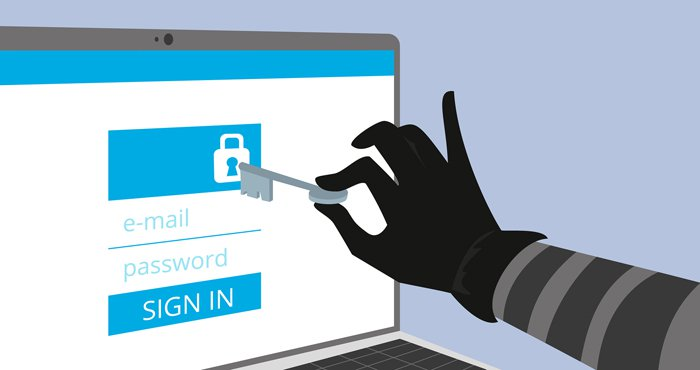
\includegraphics[width=0.3\textwidth]{Images/Monero/account.jpg}
\end{wrapfigure}
In Monero, a wallet is called an account and it is a private account owned and operated by a Monero user. An account contains all of the Monero transactions a user has sent and received. Some user's account balance is a sum of all the Monero received, less the Monero sent.

A Monero account has two balances, a locked and an unlocked balance. The unlocked balance contains funds that can be spent immediately, and the locked balance contains funds that can't be spent right away. A Monero user may receive a transaction that has an unlock time set, or he/she may have sent some Monero and are waiting for the change to come back to his/her wallet, both situations that could lead to those funds being locked for a time.

An account resides only under user's control, normally on his/her computer, and cannot be accessed by anyone else if he/she practices good security~\cite{getmonero}.

\subsection{Keys}
%\setlength{\intextsep}{0pt}
\begin{wrapfigure}[5]{L}{0.2\textwidth}
\centering
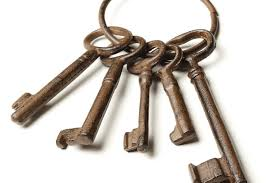
\includegraphics[width=0.2\textwidth]{Images/Monero/keys.jpg}
\end{wrapfigure}
A Monero account is based on two keys. They are called \emph{spend key} and \emph{view key}. The \emph{spend key} is special in that it is the single key required to spend your Monero funds, whereas the \emph{view key} allows you to reveal your transactions to a third party. That makes sense in case of auditing or accounting purposes.
\vspace{0.8cm}

The spine of the Monero project is the \hyperref[sec:CryptoNote]{CryptoNote} protocol. All the above specifications are based on ideas that exist in the CryptoNote white paper~\cite{citeulike:14139412}. Monero is the most successful implementation of this protocol, among numerous efforts. Describing every implementation is impractical and beyond the scope of this thesis.

However, it would be an inexcusable omission not to describe the features and specifications of the CryptoNote protocol itself. For our purposes, we will illustrate the above with Monero project in mind and especially one specific element, the \hyperref[ch:cryptonight]{CryptoNight} function (see \hyperref[ch:cryptonight]{chapter}~\ref{ch:cryptonight}), which is the feature of interest in this thesis.

Unlike many cryptocurrencies that are derivatives of Bitcoin, Monero uses a proof of work mechanism to issue new coins and incentivize miners to secure the network and validate transactions. One key part, for Monero project to offer the above, is a proof-of-work algorithm called \hyperref[ch:cryptonight]{CryptoNight}, developed by the \hyperref[sec:CryptoNote]{CryptoNote} project~\cite{citeulike:14139412}. On top of typical security attributes, this algorithm is also suspected to be memory-hard. The aim of this work is to study the \hyperref[sec:memory-hard]{memory-hardness} property (see \hyperref[sec:memory-hard]{section}~\ref{sec:memory-hard}) of this algorithm.
\clearpage
\pagebreak

\section{CryptoNote} \label{sec:CryptoNote}
%\setlength{\intextsep}{0pt}
\begin{wrapfigure}{L}{0.2\textwidth}
\centering

\includegraphics[width=0.20\textwidth]{Images/CryptoNote/cryptonote.png}
\end{wrapfigure}
The \emph{CryptoNote Technology} is designed to provide some of the most innovative privacy features predicated on advanced cryptography, an egalitarian approach towards decentralization and censorship-resistance. CryptoNote, as described in the Bitcoin forum~\cite{btcforum}, is the technology that allows creation of privacy-centric cryptocurrencies. The level of anonymity provided by CryptoNote isn't possible with Bitcoin code base by design. \emph{Bytecoin (BCN)} was the CryptoNote reference implementation, and \emph{Monero (XMR)} is based on BCN's code.

The CryptoNote protocol possesses significant algorithmic differences relating to blockchain obfuscation. One of the main features of CryptoNote, are \emph{ring signatures}~\cite{citeulike:14139412} that mask sender identities by mixing and one-time keys that make transactions unlinkable. Their combined effect gives a high degree of anonymity without any extra effort on the part of the user.

Unlike Bitcoin, a user's funds are not held in the address he/she gives out to others. Instead, every time he/she receives a payment it goes to an unlinkable address generated with random numbers. When he/she decides to spend the funds in that one-time address, the amount will be broken down and the components will be indistinguishable from identical outputs in the blockchain.

For example if 556.44 XMR are sent, the protocol will break it down into 500 + 50 + 6 + 0.4 + 0.04 and a ring signature will be performed with other 500's, 50's, 6's, 0.4's, and 0.04's in the blockchain. Unlike the \emph{CoinJoin} mixing method~\cite{btcforum}, CryptoNote mixes outputs not transactions. This means no other senders need to be participating with some user at the same time or with the same amounts. Any arbitrary amount sent at any time can always be rendered fundamentally indistinguishable (a mathematical proof is given in the white paper~\cite{citeulike:14139412}).

The degree of anonymity is also a choice rather than decided by the protocol: do you want to be hidden as one among five or one among fifty? The size of the signature grows linearly as $\mathcal{O}(n+1)$ with the ambiguity, so greater anonymity is paid for, with higher fees to miners.

\subsection{Untraceable Transactions} \label{sec:untraceable}
%\setlength{\intextsep}{0pt}
\begin{wrapfigure}[7]{L}{0.22\textwidth}
\centering

\includegraphics[width=0.22\textwidth]{Images/CryptoNote/untraceable.jpg}
\end{wrapfigure}
CryptoNote cryptographic scheme relies on the cryptographic primitive called a \emph{group signature}. First presented by D. Chaum and E. van Heyst~\cite{group}, it allows a user to sign his message on behalf of the group. The idea is actually simple. After signing the message the sender provides the keys of all the users of his group. A verifier is conviced that the real signer is a member of the group but cannot be exclusively identified.

However, this primitive required a trusted third party (Group Manager) who could trace the signer. The \emph{ring signature} was introduced by Rivest et al.~\cite{ring} and it was an autonomous scheme without anonymity revocation. Based on this work various modifications arose like \emph{linkable ring signature}~\cite{link1,link2,short}, a scheme that allowed to determine if two signatures were produced by the same group member, \emph{traceable ring signature}~\cite{traceable1,traceable2}, a scheme that limited anonymity (it is possible to trace the signer of two messages) and \emph{ad-hoc group signature}~\cite{ad-hoc1,ad-hoc2}. The last scheme focuses on the arbitrary group formation. The other schemes rather imply a fixed set of members.

Based on~\cite{traceable2} with a few modifications, in CryptoNote white paper~\cite{citeulike:14139412} is presented the \emph{one-time ring signature}. They weakened the traceability property and kept the linkability. That is needed because they wanted some user's public key to appear in many foreign verifying sets and from the private key to generate a unique anonymous signature. In case of a double spend attempt, these two signatures will be linked together. However, revealing the signer is not necessary.

Ring signatures are explained below. We will start with a normal signature scheme shown in \hyperref[fig:normal_sig]{figure}~\ref{fig:normal_sig}. Reproduced from CryptoNote~\cite{cryptonote}:
\vspace{0.5cm}
\begin{figure}[H]
  \centering
  \includegraphics[width=1 \columnwidth,keepaspectratio]{Images/CryptoNote/normal_sig.png}
  \caption{Normal signature: One participant, which allows one-to-one mapping.~\cite{cryptonote}}
  \label{fig:normal_sig}
\end{figure}

In \hyperref[fig:ring_sig]{figure}~\ref{fig:ring_sig} we show the ring signature concept.
\vspace{0.5cm}
\begin{figure}[H]
  \centering
  \includegraphics[width=1 \columnwidth,keepaspectratio]{Images/CryptoNote/ring_sig.png}
  \caption{Ring signature: Only proves that a signer belongs to a group.~\cite{cryptonote}}
  \label{fig:ring_sig}
\end{figure}

The result is shown in \hyperref[fig:result]{figure}~\ref{fig:result}. The reader can think of it as decentralized and trustless mixing.
\vspace{0.5cm}
\begin{figure}[H]
  \centering
  \includegraphics[width=1 \columnwidth,keepaspectratio]{Images/CryptoNote/result.png}
  \caption{High level of anonymity in cryptocurrency transactions.~\cite{cryptonote}}
  \label{fig:result}
\end{figure}

For an example of a complete CryptoNote transaction the reader is refered to  \hyperref[sec:cryptonote_transaction]{section}~\ref{sec:cryptonote_transaction}. Due to figure's size and complexity, it was improbable for us to manage to describe this example here, without compromising readability.

\subsection{Unlinkable transactions}
First, we should clarify the problem which is solved with unlinkability. Even if a transaction is untraceable, when the receiver posts his/her public address anyone can check all his/hers incoming transactions (see \hyperref[fig:linkable]{figure}~\ref{fig:linkable}). A naive solution is to create a bunch of keys and addresses that can be sent privately to the payers (one distinct key per payer). This approach is highly problematical since:
\begin{enumerate}[label=\alph*)]
  \item Deprives the receiver of the convenience of having a single public address
  \item Implies that the default use of the structure \textbf{DOES NOT} create unlinkable transactions
\end{enumerate}
\begin{figure}[H]
  \centering
  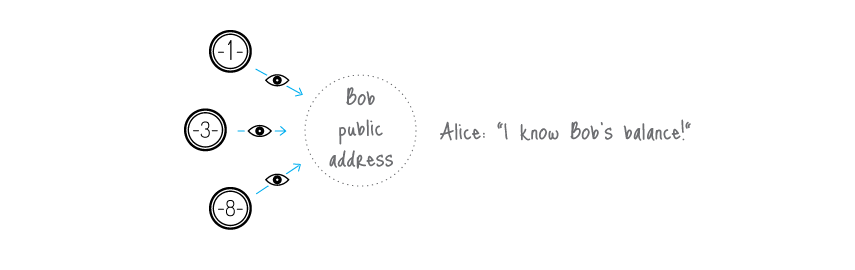
\includegraphics[width=0.9 \columnwidth,keepaspectratio]{Images/CryptoNote/linkable.png}
  \caption{Linkable transactions.~\cite{cryptonote}}
  \label{fig:linkable}
\end{figure}
\vspace{0.2cm}

CryptoNote solves this problem. It creates automatically and by default multiple unique one-time keys, derived from the single public key, for each peer-to-peer payment. The solution lies in a clever modification of the Diffie-Hellman exchange protocol~\cite{Diffie:2006:NDC:2263321.2269104}. Originally, it allows two parties to produce a common secret key derived from their public keys. In CryptoNote protocol the sender uses the receiver's public address and his own random data to compute a one-time key for the payment.

The sender can produce only the public part of the key, whereas only the receiver can compute the private part; hence the receiver is the only one who can release the funds after the transaction is committed. He only needs to perform a single-formula check on each transaction to establish if it belongs to him. This process involves his private key, therefore no third party can perform this check and discover the link between the one-time key generated by the sender and the receiver's unique public address.
\begin{figure}[ht]
  \centering
  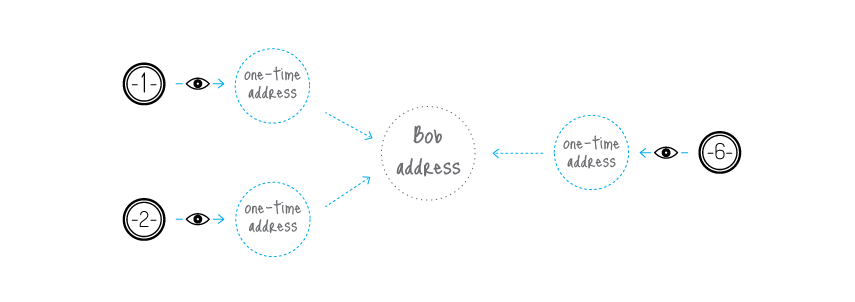
\includegraphics[width=0.9 \columnwidth,keepaspectratio]{Images/CryptoNote/unlinkable.png}
  \caption{Unlinkable transactions.~\cite{cryptonote}}
  \label{fig:unlinkable}
\end{figure}
\vspace{0.2cm}

An important part of CryptoNote is usage of random data by the sender. It always results in a different one-time key even if the sender and the receiver both remain the same for all transactions (that is why the key is called "one-time"). Moreover, even if they are both the same person, all the one-time keys will also be absolutely unique.

\subsubsection{Stealth addresses} \label{sec:stealth}
%\setlength{\intextsep}{0pt}
\begin{wrapfigure}[6]{L}{0.3\textwidth}
\centering

\includegraphics[width=0.30\textwidth]{Images/CryptoNote/stealth.jpg}
\end{wrapfigure}
The structure of the above concept is inherited in all CryptoNote projects. But the details of each implementation may differ. What we will present here is the implementation details of unlinkability, as found in the Monero project. The reader can find all the information of this section and more in CryptoNote paper~\cite{citeulike:14139412} and Monero project's code. An additional valuable source of information and interactive conversation venue that the reader is refered to is Monero stack exchange forum~\cite{stackexchange}. The implementation of CryptoNote's unlinkable transactions in Monero project is mentioned as \emph{stealth addresses} or \emph{subaddresses}.

Stealth address technology originated from CryptoNote technology, but Bitcoin (e.g. \emph{libbitcoin}) and its altcoins can also implement stealth addresses. For Bitcoin and its altcoins, stealth addresses must be explicitly supported by the sender's and recipient's wallets, but such support is implicit to CryptoNote wallets.
\begin{figure}
  \begin{verbatim}
 vJmsp9MxWMj6jiUg8Rejh23pqRCthWQhwtUKvmLw2kcE83AHer1MchTN4DVacHt
 43r8hSKBQpjPuqYDKuKgyVBkGkUdcsNAdnk2aZW
  \end{verbatim}
  \caption{Bitcoin stealth address.}
  \label{fig:btcstealth}
\end{figure}

For Bitcoin, stealth addresses are a bit longer than normal Bitcoin addresses (see \hyperref[fig:btcstealth]{figure}~\ref{fig:btcstealth}). However, the transactions associated with a stealth address looks no different than normal transactions on the Bitcoin blockchain. Stealth addresses contain one public \emph{view} (in CryptoNote vernacular) or \emph{scan} (in Bitcoin vernacular) key, and one or more \emph{spend} public keys. These keys are always encoded in a stealth address to support the first portion of Diffie-Hellman key exchange~\cite{Diffie:2006:NDC:2263321.2269104}. Bitcoin's public/private key pairs are derived from the \emph{secp256k1} elliptic curve~\cite{secg}, while CryptoNote uses \hyperref[sec:ed25519]{\emph{Ed25519}}~\cite{curve25519} (see \hyperref[sec:ed25519]{section}~\ref{sec:ed25519}) derived public/private key pairs.

One can publish their stealth address on a business card, and sustain their privacy when funds are sent to a dynamically computed destination address by the sender of funds. Stealth addresses essentially put the onus of dynamic address calculation, typically associated with a recipient's hierarchical deterministic (HD) wallet, on the sender's wallet. One stealth address is functionally akin to an HD wallet account, and can thus be used over and over for many fund transfers. Stealth addresses provide confidentiality for the recipient of transaction pairs that utilize information from a stealth address.

So, simplifying a bit, in Bitcoin if there is one Bitcoin associated to the public key $P$ and if Bob knows the corresponding private key $x$ such that $P = xG$\footnote{$G$ is the generator for the algebraic ring that is the base of the key construction. For our purpose, it suffices to think $G$ as a parameter of the user's existence in the Monero network, which is public and thus available to anyone.}, then he can spend the Bitcoin by submitting a message (transaction) to the network signed with $x$.

There is one privacy issue, though: if Bob keeps using the same $P$ to receive Bitcoins, then any observer will be able to see all payments were made to the same entity that controls $P$ (Bob). This is the problem that stealth addresses solve.
\pagebreak

Stealth addresses innately perform the first half of a Diffie-Hellman key exchange~\cite{Diffie:2006:NDC:2263321.2269104} when a sender of funds receives a stealth address. In Bitcoin, two blockchain transactions are required to complete the sending of funds to a stealth address that belongs to the recipient of funds.

Since it is operationally improbable for two users' wallets to communicate directly to each other, the first transaction is a persistent \verb|OP_RETURN| transaction that is used to complete the second half of a Diffie-Hellman key exchange. The second transaction is the actual sending of funds to a dynamically calculated destination address that is strongly based upon an ephemeral random number generator in the sender's wallet.

The second half of the Diffie-Hellman key exchange, the \verb|OP_RETURN|, allows the recipient's wallet of a stealth transaction to dynamically calculate the private redemption key associated with a particular transaction to redeem the funds at a later date.

Stealth addresses can be extended to support multisig. This is a multisig capability that is more inherent to Bitcoin than CryptoNote.

In the context of stealth addresses, addresses are now composed of two public keys, and the coins sent to Bob will not be sent to his stealth address on the blockchain, rather the stealth address will be used by the sender to produce fresh new Bitcoin addresses for every new transaction. These new addresses, even though generated by the sender (Alice) and unknown to Bob until the transaction is made, will nonetheless be controlled by Bob! Here is how it works:

Bob creates two pairs of private and public keys. Let's denote them by $(a,A)$ and $(b,B)$, where by definition
\begin{equation}
  A = aG \quad \mbox{ and } \quad B = bG
\end{equation}
Bob makes the pair of public keys $(A,B)$ available to the network; this will be his stealth address.

Alice wishes to send one Bitcoin to Bob. She wants to assign one Bitcoin to a public key $P$ such that Bob knows $x$ and $P = xG$. She will construct such $P$ using Bob's stealth address by using a hashing function $\mathcal{H}$, choosing a random big number $r$, and setting
\begin{equation}
  P = \mathcal{H}(rA)G + B
\end{equation}
Then, Alice sends the Bitcoin to $P$ and the transaction is broadcast along with $R = rG$ (but not $r$, which can't be recovered from $R$).

In order to get the money, Bob has to keep listening to the network for all new transactions and check whether one or more of these transactions are money that he should receive. When he sees Alice's transaction, he checks if $x := \mathcal{H}(aR)+b$ and realizes that:
\begin{align*} \label{eq:checkstealth}
  xG &= (\mathcal{H}(aR)+b)G \\
     &= \mathcal{H}(aR)G+bG \\
     &= \mathcal{H}(arG)G+B \\
     &= \mathcal{H}(raG)G+B \\
     &= \mathcal{H}(rA)G+B \\
     &= P
\end{align*}
\pagebreak

Bob can reconstruct $x$ such that $P = xG$ and is therefore the owner of the Bitcoin! Notice that neither Alice nor any observer has the ability to derive $x$ (because they don't know $a$ and $b$), and that besides Alice and Bob no one knows that $(x,P)$ was generated from Bob's stealth address (because they don't know $r$).

Ignoring middleman snooping on IP addresses associated with stealth address transaction pairs, only the two core parties involved in a transaction pair will know any identity details associated with sending funds to a stealth address. Hence, the need for \hyperref[sec:Kovri]{Kovri I2P technology} (see \hyperref[sec:Kovri]{section}~\ref{sec:Kovri}). So, stealth transactions by themselves don't provide 100\% anonymity protection. Also Confidential Transactions (CT) technology is needed by Bitcoin to mask details about the amount transferred by a transaction.

Note that, as mentioned, this protects Bob's privacy, but it is still visible to the network that Alice, the entity that used to control that Bitcoin, made a transaction. In order to obfuscate that action, Monero implements the use of Ring Signatures~\cite{ringCT}, which will allow Alice to, instead of directly signing the transaction, produce a proof that her or several other people, did send a coin to Bob.

To sum up, in Monero, coins are received to a unique one-time stealth address. The formula for stealth addresses, is as follows:
\begin{equation}
  P = \mathcal{H}(rA)G + B
\end{equation}
%
Where:
\begin{description}
  \item [G] The standard \emph{Ed25519} base point
  \item [A] Bob's public view key
  \item [B] Bob's public spend key
  \item [r] The new random scalar Alice chose for this transaction
  \item [$\mathcal{H}$] A hashing algorithm that returns a scalar (i.e., the hash output is interpreted as an integer and reduced modulo $l$)
  \item [P] The final stealth address (one-time output key, the destination where funds will actually be sent)
\end{description}
So, in a nutshell:
\begin{itemize}
  \item \emph{Stealth addresses} take care of \textbf{recipient's} privacy.
  \item \emph{Ring Signatures} take care of \textbf{sender's} privacy.
\end{itemize}

An \hyperref[sec:construction]{example} is presented in the \hyperref[sec:construction]{Appendix}~\ref{sec:construction} of this thesis. There, the reader can find a real world construction of a Monero stealth address.
\clearpage
\pagebreak

\subsection{Double-spending proof}
Fully anonymous signatures would allow spending the same funds many times which, of course, is incompatible with any payment system's principles. The problem can be fixed and here we reproduce the description of this solution, as presented in~\cite{cryptonote}.

A ring signature is actually a class of crypto-algorithms with different features. The one CryptoNote uses is the modified version of the \emph{traceable ring signature}~\cite{traceable2}. In fact, they transformed traceability into linkability. This property restricts a signer's anonymity as follows: if he/she creates more than one ring signature using the same private key (the set of foreign public keys is irrelevant), these signatures will be linked together which indicates a double-spending attempt.

To support linkability CryptoNote introduced a special marker being created by a user while signing, which they called a \emph{key image}. It is the value of a cryptographic one-way function of the secret key, so in mathematical terms it is actually an image of this key. One-wayness means that, given only the key image, it is impossible to recover the private key.

On the other hand, it is computationally impropable to find a collision (two different private keys, which have the same image). Using any formula, except for the specified one, will result in an unverifiable signature. All things considered, the key image is unavoidable, unambiguous and yet an anonymous marker of the private key.
\vspace{0.3cm}
\begin{figure}[H]
  \centering
  
\includegraphics[width=1 \columnwidth,keepaspectratio]{Images/CryptoNote/key_image.png}
  \caption{Key image via one-way function.~\cite{cryptonote}}
  \label{fig:key_image}
\end{figure}
\vspace{0.2cm}

All users keep the list of the used key images (compared with the history of all valid transactions, it requires an insignificant amount of storage) and immediately reject any new ring signature with a duplicate key image. It will not identify the misbehaving user but it does prevent any double-spending attempts, caused by malicious intentions or software errors.
\begin{figure}[H]
  \centering
  
\includegraphics[width=1.2 \columnwidth,keepaspectratio]{Images/CryptoNote/double_spending.png}
  \caption{Double-spending check.~\cite{cryptonote}}
  \label{fig:double_spending}
\end{figure}
\vspace{0.2cm}

\subsection{Blockchain analysis resistance}
We reproduce from~\cite{cryptonote} the reasons, why blockchain analysis in Monero project is not something that can be achieved.

There are many academic papers dedicated to the analysis of the Bitcoin's blockchain. Their authors trace the money flow, identify the owners of coins, determine wallet balances and so on. The ability to make such analysis is due to the fact that all the transfers between addresses are transparent: every input in a transaction refers to a unique output. Moreover, users often re-use their old addresses, receiving and sending coins from them many times, which simplifies the analyst's work. It happens unintentionally: if you have a public address (for example, for donations), you are sure to use this address in many inputs and transactions.

CryptoNote is designed to mitigate the risks associated with key re-usage and one-input-to-one-output tracing. Every address for a payment is a unique one-time key, derived from both the sender's and the recipient's data. It can appear twice with a probability of a 256-bit hash collision. As soon as you use a ring signature in your input, it entails the uncertainty: which output has just been spent?

Trying to draw a graph with addresses in the vertices and transactions on the edges, one will get a tree: a graph without any cycles (because no key/address was used twice). Moreover, there are billions of possible graphs, since every ring signature produces ambiguity. Thus, you can't be certain from which possible sender the transaction-edge comes to the address-vertice. Depending on the size of the ring you will guess from "one out of two" to "one out of a thousand". Every next transaction increases the entropy and creates additional obstacles for an analyst.

\subsection{More about CryptoNote}
There are several noteworthy details about CryptoNote and several implementation details of this protocol in the Monero project. However, it would be unproductive and it would harm the readability of this thesis to describe every aspect of this protocol. We believe that the reader has now a good understanding of the backbone of Monero's privacy and anonymity features. Nevertheless, before we start the \hyperref[ch:cryptonight]{CryptoNight} description (see \hyperref[ch:cryptonight]{section}~\ref{ch:cryptonight}) we will elaborate on some additional details about CryptoNote. Reproduced from~\cite{cryptonote}:

\subsubsection{Adaptive limits}
A decentralized payment system must not depend on a single person's decisions, even if this person is a core developer. Hard constants and magic numbers in the code deter the system's evolution and therefore should be eliminated (or at least be cut down to the minimum).

Every crucial limit (like max block size or min fee amount) should be re-calculated based on the system's previous state. Therefore, it always changes adaptively and independently, allowing the network to develop on it's own. CryptoNote has the following parameters which adjust automatically for each new block:
\clearpage
\pagebreak

\begin{description}
  \item [Difficulty] The general idea of our algorithm is to sum all the work that nodes have performed during the last 720 blocks and divide it by the time they have spent to accomplish it. The measure of the work is the corresponding difficulty value for each of the blocks. The time is calculated as follows: sort all the 720 timestamps and cut-off 20\% of the outliers. The range of the rest 600 values is the time which was spent for 80\% of the corresponding blocks.
  \item [Maximum block size] Let $MN$ be the median value of the last $N$ blocks sizes. Then the \emph{hard-limit} for the size of accepting blocks is $2 \cdot MN$. It averts blockchain bloating but still allows the limit to slowly grow with the time, if necessary. Transaction size does not need to be limited explicitly. It is bounded by the size of the block.
\end{description}

\subsubsection{Smooth emission}
In the CryptoNote description~\cite{cryptonote} one can find the following; the upper bound for the overall amount of all digital coins is also digital:
\begin{equation}
  \mbox{MSupply } = 264 − 1 \mbox{ atomic units}
\end{equation}

This is a natural restriction based only on implementation limits, not on intuition like "$N$ coins ought to be enough for everybody". To make the emission process smoother, CryptoNote uses the following formula for block rewards:
\begin{equation}
  \mbox{BaseReward } = (\mbox{MSupply } - A) >> 18
\end{equation}
where $A$ is amount of previously generated coins. It gives a predictable growth of the money supply without any breakpoints.

During our research, we found the above description peculiar and confusing. After a while and some forum conversations, we understood that the actual implementation restriction is that a single output cannot have an amount greater than $2^{64} − 1$ atomic units (which is $1.84 \cdot 10^{31}$ XMR).

Therefore the restriction that the above feature is refering to, is about individual outputs and not the total sum of all outputs that can exist on the blockchain.
\vspace{0.2cm}

This is currently an implementation limitation related to Monero's \hyperref[sec:bulletproofs]{\emph{bulletproofs}}~\cite{getmonero} (see \hyperref[sec:bulletproofs]{section}~\ref{sec:bulletproofs}) which proves that amounts are not negative, by proving they are less than $2^{64}$. Because Monero units are expressed as positive integers which are subject to modular arithmetic, a very high number can be equivalent to a negative number when added to another Monero amount, which is why this "less than" check proves the number is not effectively negative.

It's easy for this limit to be increased, if necessary, in the future (it's extremely unlikely to be necessary). Note that this observation is specifically related to theoretical limitations. It may be possible that certain Monero wallet implementations also store amounts using a data storage technique that would prevent numbers larger than $2^{64}$ from being stored.
\clearpage
\pagebreak

\section{Monero vs CryptoNote}
The reader understands now that the backbone for Monero's anonymity and privacy features is CryptoNote protocol. However, there are some differences. One that was already pointed out is the \hyperref[sec:stealth]{\emph{stealth address}} feature. We have noted in \hyperref[sec:stealth]{section}~\ref{sec:stealth} that the Monero stealth address implementation is unique. Other CryptoNote projects do not share exactly the same calculations.

Moreover, Monero is actively developed as it is one of the most successful cryptocoin projects and several additions have been made since its first introduction to the world. Its backbone is still the CryptoNote protocol but in this section we will mention additional features that strengthen the anonymity and privacy goals of the project.

\subsection{RingCT}
In the \hyperref[sec:untraceable]{Section}~\ref{sec:untraceable} we mentioned \emph{one-time ring signatures} that were presented in CryptoNote white paper.

In 2015, Shen Noether wrote a paper using a technique, introduced by Bitcoin Core developer Gregory Maxwell in~\cite{elements}, of using a commitment scheme to hide the amount of a transaction. The paper, introduced \emph{RingCT (Ring Confidential Transactions)}~\cite{ringCT}. This signature scheme is called \emph{A Multi-layered Linkable Spontaneous Anonymous Group signature} and that is how transaction amounts are hidden in Monero. Reproducing from~\cite{getmonero}:

\begin{verbatim}
  RingCT was implemented in block #1220516 in January 2017.
  After September 2017, this feature became mandatory for all
  transactions on the network.
\end{verbatim}
For further information the reader is refered to Shen Noether's paper~\cite{ringCT}.

The transaction structure remains similar to the structure in \hyperref[sec:Bitcoin]{Bitcoin}: every user can choose several independent incoming payments (transactions outputs), sign them with the corresponding private keys and send them to different destinations. Contrary to Bitcoin’s model, where a user possesses unique private and public keys, in the proposed model a sender generates a one-time public key based on the recipient’s address and some random data.

In this sense, an incoming transaction for the same recipient is sent to a one-time public key (not directly  to a unique  address) and only the recipient can recover the corresponding private part to redeem his funds (using his unique private key). The recipient can spend the funds using a ring signature, keeping his ownership and actual spending anonymous.
\clearpage
\pagebreak

\subsection{Bulletproofs} \label{sec:bulletproofs}
%\setlength{\intextsep}{0pt}
\begin{wrapfigure}[7]{L}{0.2\textwidth}
\centering
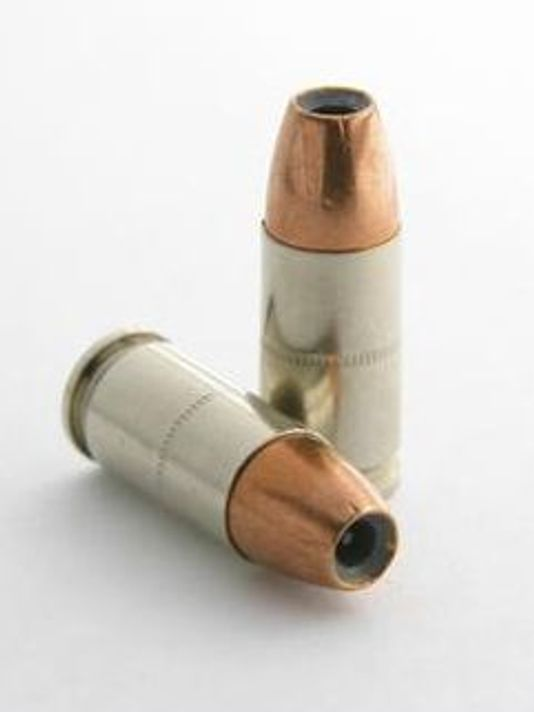
\includegraphics[height=0.23\textwidth]{Images/Monero/bullet.jpg}
\end{wrapfigure}
Starting in 2018, Monero began testing yet another highly sophisticated piece of cryptographic magic: \emph{bulletproofs}~\cite{bulletproofs}. This technology is intended to address one of the main drawbacks of \emph{RingCT}~\cite{ringCT}: the size of the \emph{zero-knowledge range proofs} this scheme produces. \emph{Bulletproofs} are a big deal, as they can increase the privacy of digital currency transactions and at the same time dramatically decrease their size. The scalability of confidential transactions have been a significant hurdle for the \$1 billion blockchain, with users long suffering high transaction fees as well as an ever-increasing cost of storage for running a full node.

\subsubsection{History}
After working on the \emph{Confidential Transactions} scheme~\cite{ringCT}, Greg Maxwell, Andrew Poelstra and Pieter Wuille teamed up with researchers from the Stanford Applied Cryptography Group to make it more efficient. Their research focused on applying a \emph{non-interactive zero knowledge proof (NIZKP)} system~\cite{0_knowledge} to aggregate all the range proofs of a Confidential Transaction and collectively prove their validity.

For context, the basic concept behind a zero-knowledge proof is to cryptographically prove that something exists, without knowing what that something is. This is achieved through a set of challenges that, if completed successfully, can statically prove that a party has a secret, without knowing what that secret is. This is the technology employed by Zcash~\cite{zcash} to entirely shield senders, receivers and the amount of ZEC (Zcash cryptocoin) sent in a transaction.

Zero-Knowledge proofs are an amazing and counter-intuitive cryptographic concept, first proposed by Goldwasser, Micali and Rackoff~\cite{0_knowledge} in a paper that introduced the idea of \emph{interactive proof} systems. The literature is extensive and if the reader wants to learn about the more modern and practical references and implementations, he/she can find the ZKP Science website~\cite{zkp_science} very useful.

The NIZKP system proposed by the bulletproof white paper~\cite{bulletproofs} has both benefits and drawbacks. On one hand, the use of \emph{NIZKP bulletproofs} does not require a trusted setup for parameter generation, like Zcash’s Powers of Tau ceremony~\cite{powers_of_tau}. On the other hand, the verification of a bulletproof is more time consuming.

\subsubsection{Details}
In order to understand bulletproofs, the reader needs to understand what a \emph{range proof} is. According to~\cite{getmonero}:
\begin{verbatim}
  A range proof allows anyone to verify that a commitment
  represents an amount within a specified range, without
  revealing anything else about its value.
\end{verbatim}

Monero uses a range proof in RingCT~\cite{ringCT} to secure the amount being sent in a transaction. Without range proofs, the amount sent could be hidden, but a sender could cheat by making coins out of thin air. Range proofs prevent this from happening. Bulletproofs achieve this goal more efficiently.
\pagebreak

\noindent From the whitepaper~\cite{bulletproofs}:
\begin{verbatim}
  [...] a new non-interactive zero-knowledge proof protocol
  with very short proofs and without a trusted setup; the
  proof size is only logarithmic in the witness size.
  Bulletproofs are especially well suited for efficient
  range proofs on committed values [...]
\end{verbatim}

Beyond improving the privacy assumptions within confidential transactions~\cite{ringCT}, bulletproofs have a much lower fingerprint (or size) relative to the proof systems used in blockchain networks today. In fact, much like \emph{SegWit}~\cite{segwit}, bulletproofs can be seen as an approach to vertical scalability as they can greatly decrease the size of a cryptographic proof from over 10kB to less than 1kB.

The bulletproof white paper~\cite{bulletproofs} focused on applying NIZKPs to the Bitcoin blockchain and stated that, if implemented, total size of Bitcoin’s UTXO\footnote{Unspent Transaction Output. UTXOs are processed continuously and are responsible for beginning and ending each transaction. Confirmation of transaction results lies in the removal of spent coins from the UTXO database. But a record of the spent coins still exists on the ledger.~\cite{investopedia}} set would be only 17 GB (compared to 160 GB) if confidential transactions were to be implemented.

It’s worth noting that bulletproofs don’t actually contribute to privacy itself. Rather, they simply ensure that the information stored within a confidential transaction doesn’t contain any false information. Pseudonymous Monero cryptographer Sarang Noether, who assisted with the bulletproofs integration, told CoinDesk~\cite{coindesk}:
\begin{verbatim}
  They’re not about anonymity; they are about assuring that
  the other stuff we do for anonymity works correctly.
\end{verbatim}

Under the previous range proof format, the size of XMR transactions scale mostly linearly depending on the number of outputs (1 output = 7kB, 2 outputs = 13kB). Under bulletproofs, transaction sizes scale logarithmically instead (1 output = 2kB, 2 outputs = 2.5kB). The size of a bulletproof increases only logarithmically with both the size of the range and the number of outputs. Reproducing from~\cite{getmonero}:
\begin{verbatim}
  This gives us two related types of bulletproofs: single-output
  and multiple-output. A transaction with multiple outputs can
  either include several single-output proofs or one multiple-output
  proof (which is smaller than the separate proofs).
\end{verbatim}

Therefore, this technology has the potential to greatly contribute to Monero’s scalability. However, one problem arose. Again, reproduced from~\cite{getmonero}:
\begin{verbatim}
  [...] an attacker could pack a transaction with many outputs;
  this tiny transaction would require low fees but would be
  computationally expensive to verify, opening the door to
  denial-of-service attacks. Because of this, we will need to
  adjust the fee structure away from transaction size and take
  into account the verification scaling.
\end{verbatim}
They explain that this means that the fees will scale properly and in a safe way. It does not mean that fees go up.
\pagebreak

The space savings granted by bulletproofs may also enable the implementation of additional obfuscation mechanisms. It is noteworthy that increasing the mandatory number of outputs in a transaction can make it significantly harder to trace balances by analyzing the blockchain. Decoys are used in ring signature inputs, but not in a transaction’s outputs. Implementing a system of decoy outputs will certainly increase the size of a transaction but this increase may be trivial post bulletproof activation.

\subsubsection{The impact}
Transaction fees on Monero, the \nth{10} largest cryptocurrency network, have fallen sharply. Bulletproofs technology made the Monero network’s privacy features more scalable by restructuring how its confidential transactions are verified.

According to data published by \emph{BitInfoCharts}~\cite{bitinfocharts}, average Monero fees fell from about \$0.54 cents to roughly \$0.021 cents in two days, a 96\% drop. Monero’s average transaction size is now 3kb versus a pre-fork average of 18.5kb. In \hyperref[fig:bulletproof_2]{figure}~\ref{fig:bulletproof_2} we can see the transaction size decrease since the implementation of bulletproofs.
\vspace{0.3cm}
\begin{figure}[H]
  \centering
  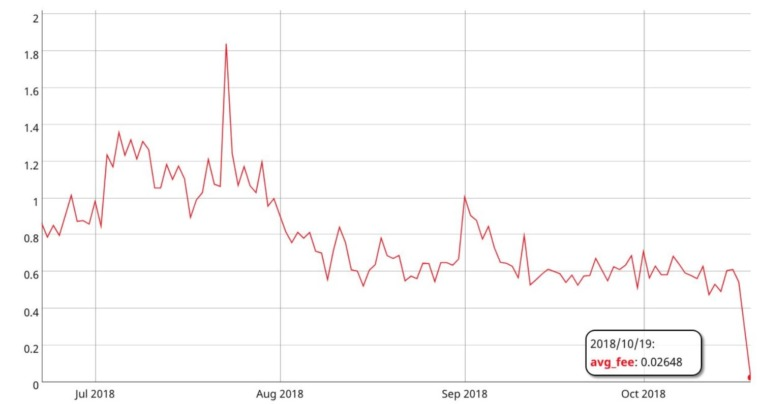
\includegraphics[width=0.8 \columnwidth,keepaspectratio]{Images/Monero/bulletproofs_2.jpg}
  \caption{July 2018 - October 2018.~\cite{bitinfocharts}}
  \label{fig:bulletproof_2}
\end{figure}
\vspace{0.3cm}
If we see this change in a broader time interval, the result is even more impressive:
\vspace{0.3cm}
\begin{figure}[H]
  \centering
  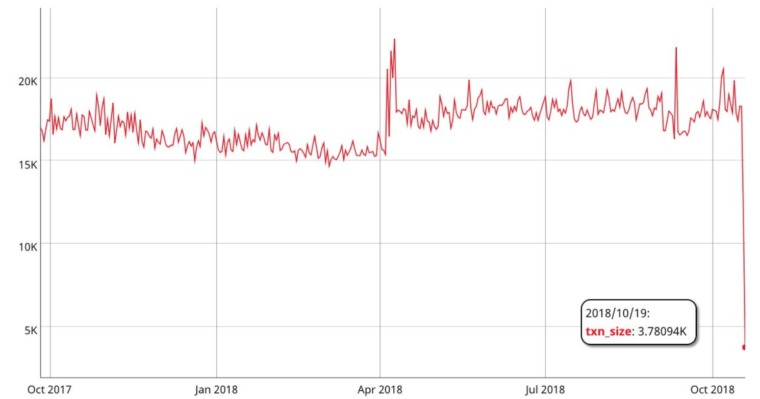
\includegraphics[width=0.8 \columnwidth,keepaspectratio]{Images/Monero/bulletproofs_1.jpg}
  \caption{July 2018 - October 2018.~\cite{bitinfocharts}}
  \label{fig:bulletproof_1}
\end{figure}
\pagebreak

There were predictions that the drop of fees might open the door to additional uses for XMR, the cryptocurrency that powers the Monero blockchain. Core developer \verb|hyc| said that the upgrade,
\begin{verbatim}
definitely [makes] the notion of micropayments more palatable again
\end{verbatim}
%%%%%%%%%%%%%%%%%%%%%%%%%%%%%%%%%%%%%%%%%%%%%%%%%%%%%%%%%%%%

\subsection{Kovri I2P Network} \label{sec:Kovri}
%\setlength{\intextsep}{0pt}
\begin{wrapfigure}[9]{L}{0.3\textwidth}
\centering

\includegraphics[height=0.28\textwidth]{Images/Kovri/kovri.jpg}
\end{wrapfigure}
Up to now, we have covered how Monero obfuscates information stored on the blockchain. Ring signatures obscure the sender. Stealth addresses prevent outside observers from knowing the receiving address. Finally, confidential transactions hide the amount of Monero transmitted. However, some personally identifiable information may be leaked at the network level when making a transaction. This privacy leak is addressed with Kovri~\cite{kovri}.

Kovri is a free, decentralized, anonymity technology based on I2P's open specifications~\cite{i2p}. Kovri uses both encryption and sophisticated routing techniques to create a private overlay-network across the Internet. This protected overlay allows users to hide their geographical location and IP address.

\subsubsection{Examples}
In the presentation of the project in the Gitlab page~\cite{git_kovri} some examples that Kovri's usage protects a user's privacy are described. These examples will help the reader to understand the significance of Kovri's contribution to the anonymity level that Monero project aims to offer. Let's reproduce here these examples.

%\setlength{\intextsep}{0pt}
\begin{wrapfigure}[5]{R}{0.3\textwidth}
\centering

\includegraphics[height=0.15\textwidth]{Images/Kovri/trace.jpg}
\end{wrapfigure}
Suppose Alice wants to send Monero to Bob. Alice's wallet creates a transaction and then broadcasts it to the Monero network. The Monero network is made up of nodes that communicate with each other by directing messages using IP addresses. This means that it might be possible to geographically trace data as it travels over the open Internet, from start to finish and everywhere in between. Even though the sender's and recipient's wallet addresses - as well as the amount of Monero sent - remain private, Alice is taking a risk in broadcasting her transaction as some nodes may be logging IP addresses. An adversary with enough resources could attempt to associate transactions with IP addresses to determine from where transactions originate. This could potentially lead to an adversary not relaying her transactions to the rest of the network; or arriving at her front door!

Now let’s imagine a different scenario. Suppose Charlie wants to support the Monero network by running a full node at his home. After a few weeks, he receives a cease and desist letter from his Internet Service Provider claiming that running a node is a violation of the terms of service.

Or consider this, suppose Dave is an operator of a mining pool that donates a portion of block rewards to a political party or controversial cause. Other nodes could purposefully reject his solved blocks to express their disagreement with his political or social views.
\pagebreak

Alice, Bob, Charlie, and Dave all have at least one thing in common: their IP addresses were exposed. Users could try to hide IP addresses with the Tor~\cite{tor} or a VPN; however both of these strategies have serious weaknesses. The Tor network has "semi-trusted" Directory Authorities which give a handful of Tor node operators overreaching influence into network consensus. Network consensus ultimately determines who is allowed to relay traffic on the Tor network based on the views of the Directory Authorities. Furthermore, correlation attacks are easily possible with trusted VPNs, making it easy for large attackers to de-anonymize a user's traffic.

If Alice, Bob, Charlie, and Dave exclusively use Kovri to connect to the Monero network, no one will know their IP address, making passive surveillance impractical, while substantially improving Monero's censorship resistance.

\subsubsection{Technical Attributes}
%\setlength{\intextsep}{0pt}
\begin{wrapfigure}[7]{L}{0.2\textwidth}
\centering

\includegraphics[height=0.20\textwidth]{Images/Kovri/doll.png}
\end{wrapfigure}
Kovri tunnels traffic through the I2P network utilizing \emph{garlic encryption} and \emph{garlic routing}. The reader can find more about this technology in the I2P Network description~\cite{i2p}. Information travels within a private overlay-network by way of messages, which are encrypted in layers each time the message is passed along to peers in the network, similar to a Matryoshka doll.

For each inner doll there is a lock and public key to the next doll. Peers in the network are not able to read the contents of the message being relayed, so information sent from the sender to its destination (and vice-versa) are secured. The only information visible to peers is the instruction for sending messages to the next peer. To achieve greater privacy at a slight cost to performance, users are able to connect to several peers.

Essentially, Kovri covers an application's Internet traffic to make it anonymous within the network. Given this characteristic, Kovri is a great solution for anonymously communicating over IRC, email, or accessing hidden services. As Kovri is an open source project, the reader can find its full details in the project's Gitlab page~\cite{git_kovri}.


\part{Back to decentralization}
%%%%%%%%%%%%%%%%%%%%%%%%%%%%%%%%%%%%%%%%%%%%%%%%%%%%%%
% For this chapter I need to build the figures.
% NOT done yet.
% Also need to be checked, but this will happen after
% the figure insertion.
%%%%%%%%%%%%%%%%%%%%%%%%%%%%%%%%%%%%%%%%%%%%%%%%%%%%%%
%% Still needs figures...

\chapter{Our Model} \label{ch:cryptonight}
%
\epigraph{Democracy must be something more than two wolves and a sheep voting on what to have for dinner.}{\textit{James Bovard}}
%
\section{CryptoNight Description}
In this section we will describe in detail the proposed implementation of the CryptoNight hash function. This function is used in the Monero project in order to achieve \hyperref[sec:egalitarian]{\emph{egalitarian mining}}. It is easy to understand why we characterize this implementation as \emph{proposed}, since each miner is free to use any implementation he/she can think of, as long as it produces the right result.

The first step we took, to understand how CryptoNight actually works, was reading Monero project's reviews. However, as Monero core developer \verb|smooth_xmr| has posted on reddit~\cite{reddit} when asked specifically about Cryptonight function reviews:
\begin{quoting}
  CryptoNight was extensively reviewed, though not as part of
  a "formal" review process, by Professor David Andersen who
  also wrote the current implementation of the hashing code.

  \noindent [...] stating that it would likely achieve its goals of resisting
  extreme optimizations and narrowing the performance gap between
  CPUs, GPUs, and ASICs.
\end{quoting}

We tried to find and read this review, as it would be a great start for our work. Unfortunately, as we discovered, the review was really informal and the best we could find was a post in professor David Andersen's personal blog~\cite{andersen}. There, one can find the \emph{first}, to our knowledge, graphical representation of the \hyperref[sec:second]{second stage} of the CryptoNight function (see \hyperref[sec:second]{section}~\ref{sec:second}).

Again to the best of our knowledge, this thesis is the close second.

In the proposed implementation, a scratchpad\footnote{A large area of memory used to store intermediate values during the evaluation of a memory-hard function.} is used (2MB) to ensure that the memory needed fits the size of L3 cache (per core) in modern processors. In practice, the miner should measure mining power and calculate efficiency.

In this chapter we will just show the proposed implementation of CryptoNight with a minor analysis in the last section. We will demonstrate the three stages of the computation and the role for each element. A really quick overview of these stages would be something like this:

\begin{enumerate}
  \item Initialize the scratchpad in a pseudo-random manner.
  \item Read/write operations at pseudo-random addresses. (\hyperref[sec:memory-hard]{\emph{memory-hard}} part)
  \item Use all the computations' results to produce the output.
\end{enumerate}

\section{The three stages}
Enough with the overview of the function and its history! Let's dive into it and see in detail its components as it is described in \cite{cryptonight}.

The input of this algorithm is a block and if the value of the Cryptonight function satisfies the target (see \hyperref[eq:target]{equation}~\ref{eq:target}), it is possible that this block is the next block in the blockchain.
\begin{equation}
  \label{eq:target}
  \color{Bittersweet} \mbox{Cryptonight}
  \color{black} (
  \color{RedViolet} \mbox{block}
  \color{black} )\leq
  \color{ForestGreen} \mbox{Target}
  \color{black}
\end{equation}

So, the input of the function is a block of transactions along with the necessary fields, which are specified by the Monero protocol. For our purposes, it is enough for the reader to think of the procedure as simple as it gets. We accept that the only way to meet the target is by bruteforcing. So, the miner tries many blocks as "candidates" and hopes for the best. Every time he/she "tries", he/she actually computes the Cryptonight digest for some random block and checks whether the \hyperref[eq:target]{equation}~\ref{eq:target} is satisfied.

In this section, we will present CryptoNight's inner computations graphically. The illustration of this section is the work of the UI and graphic designer, Vasilis Agiotis~\cite{bill}. His help is valuable, as the visual representation is needed. CryptoNight has a relatively complex operation sequence and our analysis requires focus on details.

\subsection{The first stage} \label{sec:first}
The first stage of the algorithm sets the initial value of the scratchpad. In order to prevent several attack schemes, the scratchpad must be initialized with data chosen in a way, which is indistiguishable from the uniform distribution. This is the goal.

We will describe the first stage in several parts and discuss the role of each part and its contribution regarding the properties of function's output. The first stage is presented graphically in \hyperref[fig:initialization]{figure}~\ref{fig:initialization}. We recommend the reader to refer to the graphical representation for clarity.
\pagebreak

\subsubsection{Description of the first stage}
To begin, let's prepare the tools:
\begin{enumerate}
  \item \label{hashing} Hash the input using Keccak~\cite{keccak} ($b=1600$, $c=512$).
  \item Choose the first 32 bytes of the final state.
  \item Interpret them as an AES-256 key.
  \item Expand them to 10 round keys.
\end{enumerate}

Keccak is the versatile cryptographic function that is most known as SHA-3. The parameter analysis and the description of their part is beyond the scope of this thesis. The reader is referred to their work.

We will consider Keccak a collision-free hash function. The next three steps produce random keys for encryption. We consider these keys random enough for the purpose of their use. They are interpreted as keys and expanded according to \cite{nla.cat-vn4183631}. Create the scratchpad:
\begin{enumerate}
  \setcounter{enumi}{4}
  \item Allocate 2097152 bytes (2MiB).
\end{enumerate}
The encryption part:
\begin{enumerate}
  \setcounter{enumi}{5}
  \item Split the bytes 64 to 191 into 8 blocks of 16 bytes each.
  \item \label{step 7} Encrypt the blocks as follows:
    \begin{verbatim}
      for i = 0..9 do:
          block = aes_round(block, round_keys[i])
    \end{verbatim}
\end{enumerate}
\begin{enumerate}
  \setcounter{enumi}{7}
  \item Fill 128 bytes of the scratchpad with the resulting blocks.
\end{enumerate}
Repeat:
\begin{enumerate}
  \setcounter{enumi}{8}
  \item With the resulting blocks run \hyperref[step 7]{step}~\ref{step 7} again.
\end{enumerate}

Each time 128 bytes are written, they represent the result of the encryption of the previously written 128 bytes. The process is repeated until the scratchpad is fully initialized.
\clearpage

\begin{figure}
  \centering
  \includegraphics[width=\columnwidth,keepaspectratio]{Images/Bill/initialization_cropped.pdf}
  \caption{Scratchpad initialization.~\cite{bill}}
  \label{fig:initialization}
\end{figure}
\clearpage

\begin{figure}[H]
  \centering
  \includegraphics[width=\columnwidth,keepaspectratio]{Images/Bill/input_stage_2_modified_cropped.pdf}
  \caption{Extracting $a$ and $b$ values.~\cite{bill}}
  \label{fig:stage2input}
\end{figure}

\subsection{The second stage (memory-hardness)} \label{sec:second}
The second stage of the algorithm uses the initialized scratchpad and two values that are computed from the hashed input of the function. Its goal is to perform computations on the scratchpad values (on all of them with high probability) and produce a final scratchpad structure that can't be computed otherwise or in stages (without huge time complexity). The memory-hardness property is satisfied if and only if there is no other way to compute the final state of the scratchpad using less memory than the size of the scratchpad. That is the overview. Let's see the details.

\paragraph{(The preparation part)} The core structure of this stage is a loop. However, before illustrating the computations that take place inside the loop, there are some computations needed for preparation and two technical clarifications.

\begin{enumerate}
  \item \label{memh: step 1} Compute the values of $a$ and $b$.
\end{enumerate}
Elements $a$ and $b$ are the two values which, along with the scratchpad, are given as input to the loop. More specifically, the first 64 bytes of the hashed input (the Keccak state) are split in two parts (32 bytes each part) and XOR-ed ($\oplus$), and the resulting 32 bytes are used to initialize variables $a$ and $b$, 16 bytes each.

In \hyperref[fig:stage2input]{figure}~\ref{fig:stage2input} the reader can see the visualization of this preparation part.
\clearpage

\begin{tcolorbox}[colback=yellow!5!white,colframe=yellow!65!black,title=\emph{Clarification 1:}]
  The reader may notice in \hyperref[fig:stage2]{figure}~\ref{fig:stage2} that the function uses a 16-byte value as an address in the scratchpad. Actually, the value is interpreted as a little-endian integer. The 21 low-order bits are used as a byte index. To ensure the 16-byte alignment, the four low-order bits of the index are cleared. This alignment is essential, as the data is read from and written to the scratchpad in 16-byte blocks.
\end{tcolorbox}
\vspace{0.2cm}

\begin{tcolorbox}[colback=yellow!5!white,colframe=yellow!65!black,title=\emph{Clarification 2:}]
  The main loop is iterated $524,288 = 2^{19}$ times. Every time, two blocks of the scratchpad are written, so with high probability, the whole scratchpad will be overwritten. In every iteration, along with the two blocks of the scratchpad, values $a'$ and $b'$ are computed, which are used as input to the next iteration.
\end{tcolorbox}
\vspace{0.2cm}

Now we are ready to describe the inner computations of the loop. We will divide this stage into parts, as it will help us later in the analysis. The number of parts are determined based on some intermediate values. We refer the reader to the graphical representation of this stage, presented in \hyperref[fig:stage2]{figure}~\ref{fig:stage2}.

Here, we note that the intermediate values are not memory requirements, as we can implement the computations with only 32 bytes of memory (for $a$ and $b$) plus the memory needed for the scratchpad. But during theoretical analysis and understanding of the function's computations, these intermediate values seem natural stops of the train of thought. So, after the \hyperref[memh: step 1]{step}~\ref{memh: step 1}:

\begin{enumerate}
  \setcounter{enumi}{1}
  \item \label{memh: step 2} Interpret the value of $a$ as a scratchpad address.
  \item \label{memh: step 3} Read from this address.
  \item Evaluate the AES function with data from \hyperref[memh: step 3]{step}~\ref{memh: step 3} and key the value of $a$.
\end{enumerate}
Let's call this intermediate value $c$. And let's add a final step to this part:
\begin{enumerate}
  \setcounter{enumi}{4}
  \item Calculate $c \oplus b$ and write the result to the address of \hyperref[memh: step 2]{step}~\ref{memh: step 2}.
\end{enumerate}
The value $c$ is passed as $b'$, part of the input of the next iteration. The second part involves another read from the scratchpad:

\begin{enumerate}
  \setcounter{enumi}{5}
  \item \label{memh: step 6} Interpret the value of $c$ as a scratchpad address.
  \item Read from this address. (We will refer to this intermediate value as $d$.)
  \item \label{memh: step 8} Multiply\footnote{The multiplication uses only the first 8 bytes of each argument, which are interpreted as unsigned 64-bit little-endian integers and multiplied together. The result is converted into 16 bytes, and finally the two 8-byte halves of the result are swapped~\cite{cryptonight}.} $c$, $d$ and add the value of $a$ to the result.
  \item Write the result of \hyperref[memh: step 8]{step}~\ref{memh: step 8} to the address of \hyperref[memh: step 6]{step}~\ref{memh: step 6}.
\end{enumerate}
This concludes the second part. The scratchpad is written twice per iteration. The only thing that is left to conclude the description of the second stage, is the computation of $a'$, part of the input of the next iteration. This is computed as follows:

\begin{enumerate}
  \setcounter{enumi}{9}
  \item Compute $d \oplus \mbox{(<the result of \hyperref[memh: step 8]{step}~\ref{memh: step 8}>) }$ to compute $a'$.
\end{enumerate}
\clearpage

\begin{figure}[H]
  \centering
  \includegraphics[width=\columnwidth,keepaspectratio]{Images/Bill/stage_2_cropped.pdf}
  \caption{The memory-hard part.~\cite{bill}}
  \label{fig:stage2}
\end{figure}

\subsection{The third stage}
The third stage of the algorithm uses the final state of the scratchpad to produce the output. During this stage AES operation is used. At first, the function extracts 10 key values from 32 bytes of the hashed input of the function, similar to the \hyperref[hashing]{step}~\ref{hashing} of the first stage. Extracting keys:
\begin{enumerate}
  \item Choose the bytes $[32...63]$ of the final Keccak state.
  \item Interpret them as an AES-256 key.
  \item \label{keys} Expand them to $10$ round keys.
\end{enumerate}
After this, the function needs a starting value. It applies XOR-operation($\oplus$) on bytes $[64...191]$ of the hashed input and the first 128 bytes of the scratchpad. Let's call these values \emph{input} and \emph{scratchpad[0]}.

\begin{enumerate}
  \setcounter{enumi}{3}
  \item \label{xor} \emph{input} $\oplus$ \emph{scratchpad[0]}.
\end{enumerate}
Now, using the first key of \hyperref[keys]{step}~\ref{keys} as key to the AES operation:

\begin{enumerate}
  \setcounter{enumi}{4}
  \item \label{encrypt} Encrypt the result of \hyperref[xor]{step}~\ref{xor}.
\end{enumerate}
Repeat the last two steps as follows:

\begin{itemize}
  \item Take the encrypted result of the last step as input.
  \item Take the next 128 bytes of the scratchpad (\emph{scratchpad[1]}).
  \item Use, as AES key, the next extracted key.
  \item Execute \hyperref[xor]{step}~\ref{xor} and \hyperref[encrypt]{step}~\ref{encrypt}.
\end{itemize}
until the last bytes of the scratchpad are used to the aforementioned operations. After the last bytes of the scratchpad are XOR-ed and encrypted,

\begin{enumerate}
  \setcounter{enumi}{5}
  \item \label{modified} Use the result to replace the bytes $[64...191]$ of the hashed input.
\end{enumerate}
We call the state of the hashed input after the above step as the \emph{modified Keccak state}. To produce the final result the function performs the next steps (see \hyperref[fig:stage3.1]{figure}~\ref{fig:stage3.2}).

\begin{enumerate}
  \setcounter{enumi}{5}
  \item Pass the \emph{modified Keccak state} through Keccak-$f$ (the Keccak permutation~\cite{keccak}).
  \item Choose the 2 low-order bits of the first byte of the \emph{modified Keccak state}.
  \item Based on these bits choose a hash function:
  \begin{align*}
     &\mbox{case 00: BLAKE-256} &
     &\mbox{case 01: Groestl-256}\\
     &\mbox{case 10: JH-256} &
     &\mbox{case 11: Skein-256}
  \end{align*}
  \item \label{output} Apply the chosen function to the \emph{modified Keccak state}.
\end{enumerate}
The result of \hyperref[output]{step}~\ref{output} is the output of the CryptoNight function. For more information about these functions, the reader is refered to the respective articles~\cite{10030667226,sha3groestl,sha3W09,sha3F+08}.

\begin{subfigures}
\begin{figure}[H]
  \centering
  \includegraphics[width=\columnwidth, keepaspectratio,natwidth=16.69cm,natheight=24.49cm]{Images/Bill/stage_3.1_cropped.pdf}
  \caption{The third stage.~\cite{bill}}
  \label{fig:stage3.1}
\end{figure}
\begin{figure}[H]
  \centering
  \includegraphics[width=\columnwidth, keepaspectratio, natwidth=16.38cm, natheight=14.31cm]{Images/Bill/stage_3.2_cropped.pdf}
  \caption{The third stage.~\cite{bill}}
  \label{fig:stage3.2}
\end{figure}
\end{subfigures}

\section{Analysis} \label{sec:analysis}
Now that we have described the way this function computes its output, we will try to build a model for our theoretical analysis. There are several assumptions that we have to make to abstract the function's operation. For this purpose, we build our model and define its security. At first, we have to focus on the part that is linked to the \hyperref[sec:memory-hard]{\emph{memory-hardness}} property (see \hyperref[sec:memory-hard]{section}~\ref{sec:memory-hard}). The reader now should have an understanding about the general purpose of each stage.

The first stage sets the scene for the memory-hardness part. We will assume that it initializes the scratchpad in a way, which is indistiguishable from the uniform distribution. It is safe to assume that, for an honest miner, the input is chosen uniformly at random as well. Our goal is to focus on the second stage, analyze it and then try to imagine, how an adversary miner can attack the memory-hardness property of this function. Due to the aforementioned assumptions we can conclude that the input of the second stage is chosen uniformly at random from its domain. Just to remember, the second stage's input is:
\begin{itemize}
  \item $a$
  \item $b$
  \item Scratchpad, from now on denoted as $SP$
\end{itemize}

\subsection{Parameters}
One of the first things that we need to do is to parametrize the input. We can't talk about complexity or security without the relative size between our objects or calculations. Moreover, this kind of analysis can help to generalize results and conclusions.

We will arbitrarily choose $n$ as symbol for the size of $a$ and fix everything else respectively. With that analysis in mind, we are fixing our language. Symbols:

\[
  \begin{array}{lcl}
    \mbox{Size of }a \mbox{: } & \: & n \\
    \mbox{Size of }b \mbox{: } & \: & n \\
    \mbox{Size of }SP \mbox{: } & \: & \beta_{n} = 2 \cdot 10^{6} \mbox{ bytes } \approx 2 \cdot n^{5} \mbox{ (polynomial)} \\
    \mbox{Value of }SP \mbox{ in address }x \mbox{: } & \: & SP_{x} \mbox{ (of size }n\mbox{)} \\
  \end{array}
\]

\subsection{AES as PRF}
The Advanced Encryption Standard (AES), also known by its original name Rijndael~\cite{Daemen99aesproposal:}, is a specification for the encryption of electronic data established by the U.S. National Institute of Standards and Technology (NIST) in 2001~\cite{nla.cat-vn4183631}.

AES is a subset of the Rijndael block cipher developed by two Belgian cryptographers, Vincent Rijmen and Joan Daemen, who submitted a proposal to NIST during the AES selection process. Rijndael is a family of ciphers with different key and block sizes.

For AES, NIST selected three members of the Rijndael family, each with a block size of 128 bits, but three different key lengths: 128, 192 and 256 bits.

AES has been adopted by the U.S. government and is now used worldwide. The algorithm described by AES is a symmetric-key algorithm, meaning the same key is used for both encrypting and decrypting the data.

In CryptoNight function AES is used for its properties as a cryptographic function. If a different key and a different input is chosen every time, then it is safe to assume that no prediction about the output of AES on this input can exist. To make this assumption more formal, we assume that AES is a \hyperref[sec:PRF]{pseudorandom function} (\hyperref[sec:PRF]{PRF}) and the seed is the key of AES.

In \hyperref[sec:PRF]{section}~\ref{sec:PRF} the reader can find the mathematical definition of PRFs. We define the notion and then we define a game. Based on this game we describe a security model to base the above assumption.

\subsection{Operations} \label{sec:operations}
Apart from the AES use, the memory-hard stage of CryptoNight function performs one addition, two XOR-operations and one multiplication. In order to be able to produce conclusions, we try to analyze what the side effects of these operations are. All of these operations get two inputs of 16 bytes size and produce a 16 byte result.

Let's examine them one by one. In the case of the XOR operation, it is easy to see that if the two inputs are chosen uniformly at random, then the result is also uniformly chosen at random. In the case of addition, reproduced from CryptoNote~\cite{cryptonight}:
\begin{quoting}
   The \verb|8byte_add| function represents each of the arguments as a
   pair of 64-bit little-endian values and adds them together,
   component-wise, modulo $2^{64}$. The result is converted back into
   16 bytes.
\end{quoting}

It is trickier to see the same here, but with a little effort one can see that if the input is chosen uniformly at random, then the result is uniformly chosen at random too. In the case of multiplication, reproduced from CryptoNote~\cite{cryptonight} again:
\begin{quoting}
   The \verb|8byte_mul| function, however, uses only the first 8 bytes
   of each argument, which are interpreted as unsigned 64-bit
   little-endian integers and multiplied together. The result is
   converted into 16 bytes, and finally the two 8-byte halves of
   the result are swapped.
\end{quoting}

The last case, is more complex. At first we notice the following: if one of the inputs is null, then the result is also null. That could be a problem. We try to calculate the probability that the result is null, due to the null value of one or both inputs. We don't care about the null value of the result due to modulo operation. That probability is obviously equal to the probability that the result is equal with some other value. We would like the "extra" probability, that the value of the result is null due to input's null value, to be negligible.

Because of the special way CryptoNight function performs the multiplication, the inputs' sizes are 64 bits = 8 bytes = $\frac{n}{2}$. In addition, considering that AES is a PRF (assumption) and $SP$ is unifomly random (at least at the first round by assumption), then the two inputs are independent. The probability of one or both inputs to be null is:
\begin{equation} \label{prob_zero}
  \frac{1}{2^{n/2}} + \frac{1}{2^{n/2}} - \frac{1}{2^{n/2} \cdot 2^{n/2}} = \frac{2\cdot2^{n/2}-1}{2^n} < \frac{1}{2^{(n/2)-1}} = \mbox{\textbf{negl}(n)}
\end{equation}
\vspace{0.3cm}

That seems to be fine for our analysis. But, the next problem is this: Multiplication of two 8 byte numbers produces a result modulo 16 bytes (mod $2^{128}$). The reader can see that the probability of a value to be an output of the multiplication declines, as the values grow. Even after the swap that is performed at the end of the multiplication, the problem persists. We have not a uniformly at random distributed result, even if the inputs are chosen uniformly at random.

The above multiplication is perfomed this way because of the modern CPU registers' size. The 8 bytes multiplication is optimized. ASICs couldn't do this as fast as a modern CPU could, but technology advances and now there are chips that do the same computation roughly with the same time cost.

However, after our theoretical analysis we think that we should propose something better. The time cost of a 16 byte multiplication or maybe an 8 byte multiplication implementation that maps inputs' uniform distribution can make a system less efficient against ASICs, compared to the official implementation proposal, but not completely inefficient. Nevertheless, this is a detail and does not make great difference in our analysis. From now on, we can assume that the above problem is solved and we have a multiplication implementation that produces a uniformly at random distributed result.

\chapter{CryptoNight Analysis}
%
% A glimpse on what set of variables are NOT independent, or NOT DEFINITELY independent. (Maybe this goes to the proof section)
%
\epigraph{Nobody can give you freedom. Nobody can give you equality or justice or anything. If you're a man, you take it.}{\textit{Malcolm X}}
%
\section{Introduction}
In order to prove that a function is \hyperref[sec:memory-hard]{\emph{memory-hard}} (see \hyperref[sec:memory-hard]{section}~\ref{sec:memory-hard}) we need to show that no implementation exists, that can produce the same result using less memory without significant time cost. In other words, using an implementation which needs less memory is not something that can give advantage to some miner because the time factor will make the procedure equally or more \emph{expensive}, even if the miner uses parallel computation techniques. Reproduced from CryptoNote~\cite{cryptonight}:
\begin{quoting}
  CryptoNight is a memory-hard hash function. It is designed to be
  inefficiently computable on GPU, FPGA and ASIC architectures.
\end{quoting}

In Monero mining, CPU's cores are only efficient if they can use the super fast 2MB cache over and over. Each core needs about 2MB for CryptoNight to stay cached. So a miner should check how much L2 cache or - in rare cases - also L3 cache the CPU has. Then divide by 2MB and this will be how many cores he/she can run at the same time.

There are several reasons to suspect that CryptoNight could be a memory-hard function. One of the most popular arguments was that a megabyte of internal memory is an almost unacceptable size for a modern ASIC pipeline. But hardware is constantly evolving and eventually there was recently an effort for Monero ASIC production. The first documented effort was the ASIC called \emph{Antminer X3} by Bitmain~\cite{bitmain}. The announcement was made in March 2018. Observing the raise of hashrate in the network, it was obvious that there were ASICs used for mining.

Founded in 2013, Bitmain, is a firm that produces ASIC chips and mines Bitcoin. The firm also operates \emph{Antpool}, which according to observers is the largest Bitcoin mining pool. An ASIC device by Bitmain has been mining Bitcoins for many years.

The reason Monero is planning to make Bitman’s Antminer X3 ineffective, is that it could enable some forms of attacks. These attacks could result in the mining pool taking over principal cryptocurrency’s hashrate. The act may enable double spending of coins, false transaction histories and censoring payments.

Riccardo Spagni, in a response to a Twitter comment which sees ASICs as a good thing~\cite{fluffypony}, said:
\begin{quoting}
  Removing all of the hashrate distributed among tens of
  thousands of miners, in favour of a handful of miners
  that can afford an overpriced machine from a single
  manufacturer is GOOD for security?
  I doubt even you believe that.
\end{quoting}

There were some thoughts like "\emph{How did they do this? Isn't CryptoNight memory-bound?}". Well, one thing is that CryptoNight is \emph{ASIC-resistant}, not \emph{ASIC-proof}\footnote{ASIC manufacturers are discouraged from building an ASIC for Monero mining, but there is no formal mathematical proof stating that an ASIC cannot be built.}. But, that was not the problem. Another thought is that L3 cache supports a lot of extra functionality like being shared across cores, writing back to RAM, being behind two other levels of cache, etc. which all makes it a lot less efficient (among other issues with the approach). But, again, that was not the case in that particular effort.

L3 latency wasn't the issue. ASICs just traded latency for bandwidth the same way GPUs do. They were built on stacks of DRAM, not lightning fast caches. The costs of cache complexity aren't only latency but also power usage and die space. Raw speed isn't even necessarily the goal for either CPUs or GPUs or ASICs here, it is efficiency.

But Monero project reacted and announced upgrades bi-annually in order to keep ASICs at bay. Upgrades are a problem, because upgrades produce bugs and vulnerabilities. Especially when they are that frequent. On the other hand, upgrades in Monero are minor, with no changes in the memory-hard part. From this experience, we understand that a formal proof, or even a better understanding of the memory-hardness property in practice, is vital for its mining function in order to protect a cryptocurrency from centralization.

\section{Proof approach}
Our starting plan was quite simple. The moment we understood the operations that took place in the computation, we had a specific strategy in mind. We would prove:

First case (\emph{honest} miner):
\begin{itemize}
  \item If the input is uniformly at random chosen, then the output is of the same nature \emph{and} independent from the input. (one round)
  \item The above expands to the whole function, not just one round.
\end{itemize}

What we wanted to show, with the two steps above, is the following: No shortcuts exist for the calculations involved. If the miner is honest, then the hash of the block will be uniformly at random chosen and so will be the elements of the input ($a$, $b$ and $SP$) of the second stage. If that implies that the output of this process is also chosen uniformly at random, then every operation on the input cannot be guessed except with negligible probability, ergo no shortcut of this process exists.

Of course, another requirement is the input ($a,b,SP$) to be independent from the output ($a',b',SP'$), where $SP'$ is the modified $SP$ after the round. If this is not the case, then there is a relation between two or more elements and in the nature of that relation a chance for an attack may hide.

It is easy to expand the above hypothetical result to the function as a whole. Every round produces a uniformly at random chosen result. Thus, the last round will produce a uniformly at random distributed result too.

Second case (\emph{malicious} miner):
\begin{itemize}
  \item If the input is \emph{not} chosen at random, then the output is \emph{still} uniformly at random chosen \emph{and} independent from the input. (one round)
  \item The above expands to the whole function, not just one round.
\end{itemize}

If we had the results for the honest case, then the next step would be to show that even if the miner is malicious he cannot do any better for himself. Even if the input is not chosen uniformly at random, the result will be distributed uniformly. That means that even if we "fixed" the input to our taste, we could not guess the result except with negligible probability. The second step follows a similar train of thought as in the case of the honest miner.

If we managed to prove the above, that would be a proof of the CryptoNight's memory-hardness property. If we cannot find a shortcut for the process, then we cannot find a way to calculate the result with less memory or less time. Let us elaborate on the details of our research.

\subsection{The model}
Based on the aforementioned plan and with help from the observations and assumptions we made in \hyperref[sec:analysis]{section}~\ref{sec:analysis}, we now use the model of computation we assume for CryptoNight's second stage (see \hyperref[fig:model]{figure}~\ref{fig:model}) to begin our analysis.

The reader can see that there is a natural division of the process in three parts. The first part is the set of all operations performed on the first address' value. Explicitly, that involves:
\begin{description}
  \item [Read] Input to an AES operation. Under our assumption, AES is a pseudorandom function (PRF).
  \item [Write] The result of a XOR ($\oplus$) operation.
\end{description}

The second part involves any operation performed on the second address' value. More precisely:
\begin{description}
  \item [Read] Store the value of the address.
  \item [Write] The result of a multiplication and an addition.
\end{description}

The third part is not of much interest for our purposes. It extracts the two outputs needed as input for next round of the second stage:
\begin{itemize}
  \item A XOR ($\oplus$) operation on the result of the addition that produces the first input of the next round ($a'$).
  \item The result of the PRF operation (AES) that is passed as the second input of the next round ($b'$).
\end{itemize}
\clearpage
%% natwidth=210mm, natheight=297mm :: A4 sizes

\begin{figure}[H]
  \centering
  \includegraphics[width=0.85\columnwidth, keepaspectratio]{Images/Bill/model_cropped.pdf}
  \caption{The model.~\cite{bill}}
  \label{fig:model}
\end{figure}

Here we note again (see \hyperref[sec:operations]{section}~\ref{sec:operations}) the special nature of the multiplication. Just for our purposes, we assume that it sustains the properties of its input. If the input (the two integers, each of size $n$) is uniformly at random chosen then the output of the multiplication is of the same nature. We strongly declare that this is not the case for the specific implementation of this operation. However, we will see that even with this assumption, we will not achieve our goal.

\subsection{The road to proof construction}
Based on the above we begin our analysis. Under the following assumptions,
\begin{itemize}
  \item $a,b$ are uniformly at random chosen
  \item AES is a PRF
\end{itemize}
we get that the first address of the round is changed in a way that does not change the distribution of the scratchpad. Everything seems fine.

For the second address we get the same result. Our assumptions are:
\begin{itemize}
  \item AES is a PRF
  \item $\forall c : SP_c$ is uniformly at random chosen
  \item Multiplication and addition sustain the distribution of their inputs
\end{itemize}

Let's see the values of $a'$ and $b'$:
\begin{align} \label{eq:normal_1}
  a' &= \Big( a + \big( PRF(a, SP_{a}) \cdot SP_{PRF(a, SP_a)} \big) \Big) \oplus SP_{PRF(a, SP_a)}\\ b' &= PRF(a, SP_{a}) \label{eq:normal_2}
\end{align}

Here we have a major problem. The problem is not the distribution of the output. Under our assumptions that is appropriate. But,
\begin{itemize}
  \item $a'$ is \emph{not} independent from $a$
  \item $b'$ is \emph{not} independent from $b$
  \item $SP'$ (scratchpad after the round) is not uniformly at random chosen
\end{itemize}
The third statement comes out of the observation that the value of $SP_a$, after the write operation, is dependent on the value of $b$. These are observations that spoil our plan.

However, this is a hint to the possibility of the existence of a successful attack on the memory-hardness property of CryptoNight function. Part of the input of this stage (values of $a,b$) is produced right from the hashed input of CryptoNight (see \hyperref[sec:first]{sections}~\ref{sec:first},~\ref{sec:second}). If someone can control the value of $a$, or maybe some bits of $a$, then he has a partial control of the value of $a'$ or at least some control over the range of $a'$. The same apply to the values of $b$ and $b'$.

This is, of course, nothing more than an intuition, so let's see if we can achieve the planning of said attack.
%% Trying the attack approach
\section{Attack approach}
The above intuition, apart from the assumptions involved, implies a level of control over the value of $a$ or $b$ or both. This can be done with grinding techniques. In a very high level of abstraction, the miner can hash the input multiple times with Keccak, changing every time something in the block (nonce, sequence of transactions, etc.). That will give him a different digest every time, ergo a different value for $a$ and $b$. This is quite efficient, especially if an ASIC is involved.

But we will make a stronger assumption. We will assume that some adversarial miner has a total control over the value of $a$ and $b$. We will show that even in that case, an attack seems impossible. Due to the nature of our results, it doesn't make sense to analyze the way an attacker can gain control over the value of $a$ or $b$.

\subsection{Details}
What is the level of impact that we can cause, if we could control the values of $a$ and $b$? What is the best we can do in order to achieve our goal?

If someone takes his/her time observing the process, he/she can see the only thing that we can hope for. That is to find an address $a$, with a content $SP_a$ such that:
\begin{equation} \nonumber
  \mbox{AES}(a,SP_a) = a
\end{equation}

The reader can see the visualization of this scenario in \hyperref[fig:attack]{figure}~\ref{fig:attack}. Now it is time to measure the probability of this event. If this probability is negligible, we cannot find anything more that we can do. We have $\beta_n$ addresses on the scratchpad and in the CryptoNight description~\cite{cryptonight} we see that:
\begin{quoting}
  When a 16-byte value needs to be converted into an address in
  the scratchpad, it is interpreted as a little-endian integer,
  and the 21 low-order bits are used as a byte index. However,
  the 4 low-order bits of the index are cleared to ensure the
  16-byte alignment.
\end{quoting}

This means that, for a uniformly at random chosen 16-byte number, the probability for the value to be converted into a specific address in the scratchpad is:
\begin{equation} \nonumber
  \frac{1 \cdot \mbox{\textbf{sizeof}}(\mbox{address})}{\mbox{\textbf{sizeof}}(SP)} =
  \frac{1 \cdot n}{\beta_n} = \frac{n}{2 \cdot n^5} = \frac{1}{2 \cdot n^4} = \frac{1}{\mbox{\textbf{poly}}(n)}
\end{equation}

That is, for all intents and purposes, \emph{not} a negligible probability with respect to the size of $n$. Hence, that is something that we can do efficiently enough. Let's see what this scenario gives us, as a round outcome. If the reader cares to do some math, he/she will see that \hyperref[eq:normal_1]{equations}~\ref{eq:normal_1},~\ref{eq:normal_2} become:
\begin{align} \nonumber
  a' &= \Big( a + \big( a \cdot (a \oplus b) \big) \Big) \oplus (a \oplus b) &
  &\mbox{and} & b' &= a
\end{align}

This looks really promising. Until we see what happens to the next round. The one thing that the reader is suggested to observe is that, although $a'$ is a function of $a$ and $b$, it is certainly not equal to either of them.

In the next round, the value $a'$ will point to a different location on the scratchpad ($SP_{a'}$) and the value $\mbox{PRF}(a', SP_{a'})$ will point to a random address in the scratchpad. And this is exactly the moment we lose the control we had over the process.
\clearpage

\begin{figure}[H]
  \centering
  \includegraphics[width=\columnwidth, keepaspectratio]{Images/Bill/attack_cropped.pdf}
  \caption{The attack scenario.~\cite{bill}}
  \label{fig:attack}
\end{figure}

\chapter{Conclusion}
%
\epigraph{Arguing that you don't care about the right to privacy because you have nothing to hide is no different than saying you don't care about free speech because you have nothing to say.}{\textit{Edward Snowden}}
%
\section{Summary}
The intuition behind the nature of the problem lies in the relation between the first and the second address written in each loop, in the second stage of the function. As we saw, the first address is a random pointer produced from the input. This is something that can be leveraged to some adversary's advantage, at least in the first round. But the way the second pointer is produced makes it hard to keep track of the computation.

Now, let's take a step back. If we want to attack the memory-hardness property, what exactly is our goal? Well, the train of thought is the following: If we managed to compute the first 128 sequential bytes of the state of the scratchpad (after the second stage), without using the rest of it, then it would be a win. We can compute in steps the digest of the CryptoNight function, using just 128 bytes of the scratchpad in each step.

We can calculate the initialization of the first 128 bytes of the scratchpad, then move on to the second stage and finally compute the first part of our solution, running just the first step of the third stage. Then, we repeat the above for every other 128 bytes of the scratchpad (15,625 times). This will give us the digest of the function, using 256 bytes of memory (2$\cdot$128, in order to remember last round's outcome) and time complexity of the same order of magnitude as the proposed implementation. That would complete a successful attack.
\pagebreak

The reason we failed is that it seems impossible to control the pointers to the addresses in the second stage. We cannot compute the final stage of the scratchpad, 128 bytes at a time. We need all of it to produce a correct computation. Let's see the details.

Without loss of generality, let the first address be $a$ and the second address be $b$, within some loop. Then,
\begin{equation} \nonumber
  b = AES(a,SP_a)
\end{equation}

Under the assumption that AES is a PRF, the above can be leveraged as we described but for one round at most. Then, control is lost. The reason is that the output of a PRF cannot be guessed with more than negligible probability. That means that we can't control the sequence of the addresses written in the second stage. Thus, we can't compute partially the final stage of the scratchpad. It has to be used as a whole.

\section{Future Work}
At first, our intuition was that the next step towards the goals of this thesis is to analyze the relation between the inputs and the outputs in each round. Maybe there is something there, we could not find. But with a closer look, it seems that if we cannot "fix" the relation to the equality one, then any control we might achieve by this analysis is lost in the next round, due to our assumption that AES is a PRF.

It is obvious that a successful attack on the AES function could lead to a successful attack on CryptoNight's memory-hardness property. However, AES being a PRF, is a reasonable assumption and it is expected to be hard to find a vulnerability in AES and a distinction between AES and PRFs. AES is a cryptographic primitive that has been thoroughly reviewed and checked.

We don't know yet, whether the reverse is true. Namely, whether a successful attack on CryptoNight's memory-hardness property is a step towards a successful attack on AES. This is a step that can follow our work, but it seems a really tricky and difficult problem.

\subsubsection{Fresh point of view}
If someone wants to continue our research, we recommend a huge step back. Maybe another model for the problem or something that is not produced from a similar point of view. As we presented in this thesis, we have found problems very early in our analysis and we couldn't pass beyond the second round of the second stage.

If someone wants to perform a cryptographic analysis on CryptoNight's memory-hardness property, then he/she is supposed to analyze this second stage. This second stage is the place where the origins and the basis of the memory-hardness property lie.
\clearpage
\pagebreak

\section{Epilogue}
This thesis is the first, to our knowledge, to analyze the memory-hardness property of the CryptoNight function. We hope that our analysis is helpful to the researcher or the researchers, who would like to continue this effort. We tried to make this document a good start for further exploration of this interesting and valuable problem.

We wish good luck to the people that will continue this work and help the Monero community in their effort for a better world. Surveillance amplification in the physical and digital world is apparent in our days and we believe that progress in research for anonymity and privacy in the public domain is something that many people seek. After all, privacy is a fundamental human right that many - if not all - human rights are based on. Without privacy, human rights, i.e., \emph{freedom of speech}, collapse.

%
%
%
%% End of the document, clear page and prepare for bibliography
%
\cleardoublepage
\phantomsection
\addcontentsline{toc}{chapter}{Bibliography}
%
%
%% Bibliography
%
\printbibliography[filter=papers,title={Bibliography}]

\printbibliography[heading=subbibintoc,type=misc,title={Web resources}]

\end{document}
